\section{Intuition of Task2Vec}
\label{appendix:intuitiontask2vec}
To better understand Task2Vec embeddings, observe that the (diagonal) of the FIM can be interpreted as a measure of the information that a given parameter contains about the generative distribution $p_w(\hat x_t \mid x_{t-1:1})$. 
Therefore, it serves as a unique fingerprint, or feature vector, for a batch, which defines a task distribution; as such, this vector, in its entirety, is as large as the number of parameters of the probe network.
Empirical findings in \citep{task2vec} show that Task2Vec embeddings cluster in a way that reflects semantics between different visual concepts, and that Task2Vec cosine distances are positively correlated with taxonomical distances.

We will provide a rephrasing from the original Task2Vec \cite{task2vec} explaining why Task2Vec is captures the importance of the weights and therefore why it serves as a unique fingerprint for a task.
The importance of a weight in a network can be measured by how much the predictions changes (average KL divergence of the original vs perturbed output) with respect to the loss of interest to target task.
Consider a perturbation of the weights $w' = w + \delta_w$.
This is the a 2nd-order approximation to the change in outputs:
$$
E_{x ~\sim \hat{p}}[KL(p_w' || p_w)] = \delta_w F \delta_w^\top + o(\delta(w)^2)
$$
Therefore, the information content of the weights is measured by this change in output captured by the Fisher Information Matrix.
Therefore, this serves as a unique finger-print of which parameters are important, making the diagonal of F a strong candidate for the unique fingerprint of a task via importance of weight.
For a relation between Task2Vec and Kolmogorov Complexity, see section \ref{kolmogorov_fisher_relation}.

\section{Related Work (cont.)}\label{related_work_cont}

% Other approaches to data-centric Machine Learning involve efficiently cleaning datasets by pruning pre-training datasets through the discard of weak examples, aiming to disrupt the power-law relationship between loss and performance \citep{abbas2024effective} \cite{}

Building on the success of deep learning data representations, we demonstrate deep learning is a strong way to create dataset/task embeddings.
In contrast to the Vendi Score, our approach learns effective embeddings of datasets in an end-to-end manner, whereas the Vendi Score is focused on measuring diversity between specific data points. 
Since many datasets are publicly available (e.g. Common Crawl, Wikipedia), data used to train new models may be curated from such datasets, necessitating a metric that captures overall data diversity.
These scenarios are thus in favor of using the Task2Vec diversity coefficient. 
Therefore, our method is likely more general and scalable than the Vendi Score. 
We leave a detailed comparison with the Vendi Score as future work.

Returning to the utility of a practical diversity metric, there is strong empirical support from efforts at increasing multi-modal image and text data quality that using \textit{semantically} deduplicated data (as opposed to simply exact \textit{match} deduplication) for training can yield impressive training efficiency gains and even improve out of domain generalization \citep{abbas2023semdedup, abbas2024effective}. Though motivated by the same underlying hypothesis about the importance of diversity in data quality, our work on the diversity coefficient focuses on text-only data, the standard for training LLMs, and yields a more interpretable metric that allows practitioners to rigorously \textit{understand} the quality of datasets, enabling the informed \textit{choice} of baseline higher quality datasets rather than only being able to \textit{improve} a \textit{chosen} dataset. Furthermore, the generality of the diversity coefficient allows it to assess and inform the results of traditional data \textit{pruning}, which has been shown to be a promising method for increasing data quality \citep{sorscher2023neural}, while also lending itself naturally as a useful metric for guiding diverse data corpora \textit{construction}, which has also been seen to be a fruitful endeavor with the release large, diverse, open source corpora \citep{thepile}.

More generally, better understanding and clarity about the characteristics of datasets and data quality enable greater control and direction of model capabilities \citep{mitchell2023measuring}, which become especially important as models become more complex, more powerful, and more important to scientific and economic activity. 

However, the benefits of this more sophisticated aggregation method are not clear, and its computation ($O(n^3)$) is more expensive than the diversity coefficient ($O(n^2)$). 
Moreover, it assumes a suitable similarity function/kernel, and does not provide guidance on data representation, arguably the most important ingredient in machine learning. 
Furthermore, they suggest that utilizing data representational methods such as embedding networks that require pretrained models may be limiting.
We argue instead that data representation is a fundamental property of data processing that has led to the overwhelming success in machine learning due to deep learning, e.g. in computer vision \citep{alexnet, resnet}, natural language processing \citep{bert, gpt3, chowdhery2022palm, gpt4, google2023palm2}, game playing \citep{alphago, atari1, EfficientZero}, theorem proving \citep{skiptree, gptf, pact}, code \citep{codex} and more.
For further comments on the Vendi Score see section \ref{related_work_cont}.

\section{Justification of Task Based (Task2Vec) Diversity vs Activation, Token, and Model Agnostic based Diversity Formalizations}
One could potentially have used different data and task representations to formalize diversity.
In this section, we explain the reasons for using Task2Vec compared to other reasonable representations. 
We explain it compared to 3 potential alternatives: 
1. Activations as data representation
2. Diversity based on token distribution
3. Model Agnostic Distributions, e.g., using Kolmogorov Complexity/minimum description lengths.

\subsection{Resolution Power Deficits in Activation-Based Diversity Approaches Compared with Task2Vec Diversity}\label{subsection:div_acts_vs_task2vec}
\textbf{Result:} 
We discover that activation-based diversity lacks the resolution to detect changes in diversity at a granular level.
We demonstrate this in figure \ref{fig:div_acts_vs_task2vec} where the activation-based diversities become flat quickly, while Task2Vec diversity (the diversity coefficient) varies more smoothly and detects diversity changes for longer. 

\textbf{Method:} The alternative definition of diversity we explored was computed by taking the average distance between a pair of batches of sequences of text and using GPT-2's final layer as the data representation of the batch:
\begin{equation*}\label{act_div}
\begin{aligned}
    \textrm{$\hat{d}$iv}(D) =
    \mathbb{E}_{B_1, B_2 \sim D} 
     % \left[ 
     d_{metric}( GPT2^{(L)}(B_1), GPT2^{(L)}(B_2) )
     % \right]
\end{aligned}
\end{equation*}
Where $B_1, B_2$ is a standard batch of text sequences, $D$ is the data distribution, $metric$ is Linear Centered Kernel Alignment (CKA) \citep{cka} or PW Canonical Correlation Analysis (PWCCA) \citep{pwcca}, $GPT2^{(L)}(B1)$ is the activation matrix of the final layer $L$ after reshaping it to size $R^{BT \times D}$ where $B$ is the batch-size, $T$ is the sequence length and $D$ is the size the final layer activations (768 for GPT2). 

\textbf{Experimental Setup: } 
We varied the size of the vocabulary size $|V|$ from $2/|V|$ to $0.4 |V|$ using 100 evenly spaced samples. 
We focused only on that range because CKA and PWCCA became flat very quickly---just after $8.09\%$ (at 0.0323), while the Task2Vec diversity did not become flat but instead followed close to a linear trend. 
The data generation distribution $D$ was uniform independently sampled random tokens. 
The batch-size $B$ was $32$ with sequence length $T$ equal to 240 and the number of batches we used for the expectation was $30$. 
We also made sure the dimensionality $D=768$ of the activation matrix was $10$ times smaller than the $TB = 240 * 32 = 7,680$. 
This last condition is crucial for CKA, PWCCA distances to not be vacuous \cite{svcca, curse_low_div}. 
Intuitively, this happens because one has more features than effective data points and say CCA tries to maximize linear correlation vectors between the two datasets that can always be done perfectly with too many features. 

\textbf{Experimental Interpretation: }
We hypothesize that Task2Vec has more resolution than activation-based diversities because Task2Vec attempts to estimate an approximately unique fingerprint of the generating parameters of the batch. 
However, activation instead has been optimized for next token prediction/discrimination (or in classical supervised learning for classification), 
i.e., features are obtained that discriminate well between data classes/vocabulary indices. 
Therefore, one would expect consistently high distances between activation-based features---which is what we approximately observe, after only $8.09\%$ of the x-axis, the activations based diversity (average activation distance) achieves the maximum value and remains constant.  

\begin{figure*}[h]
    \centering
    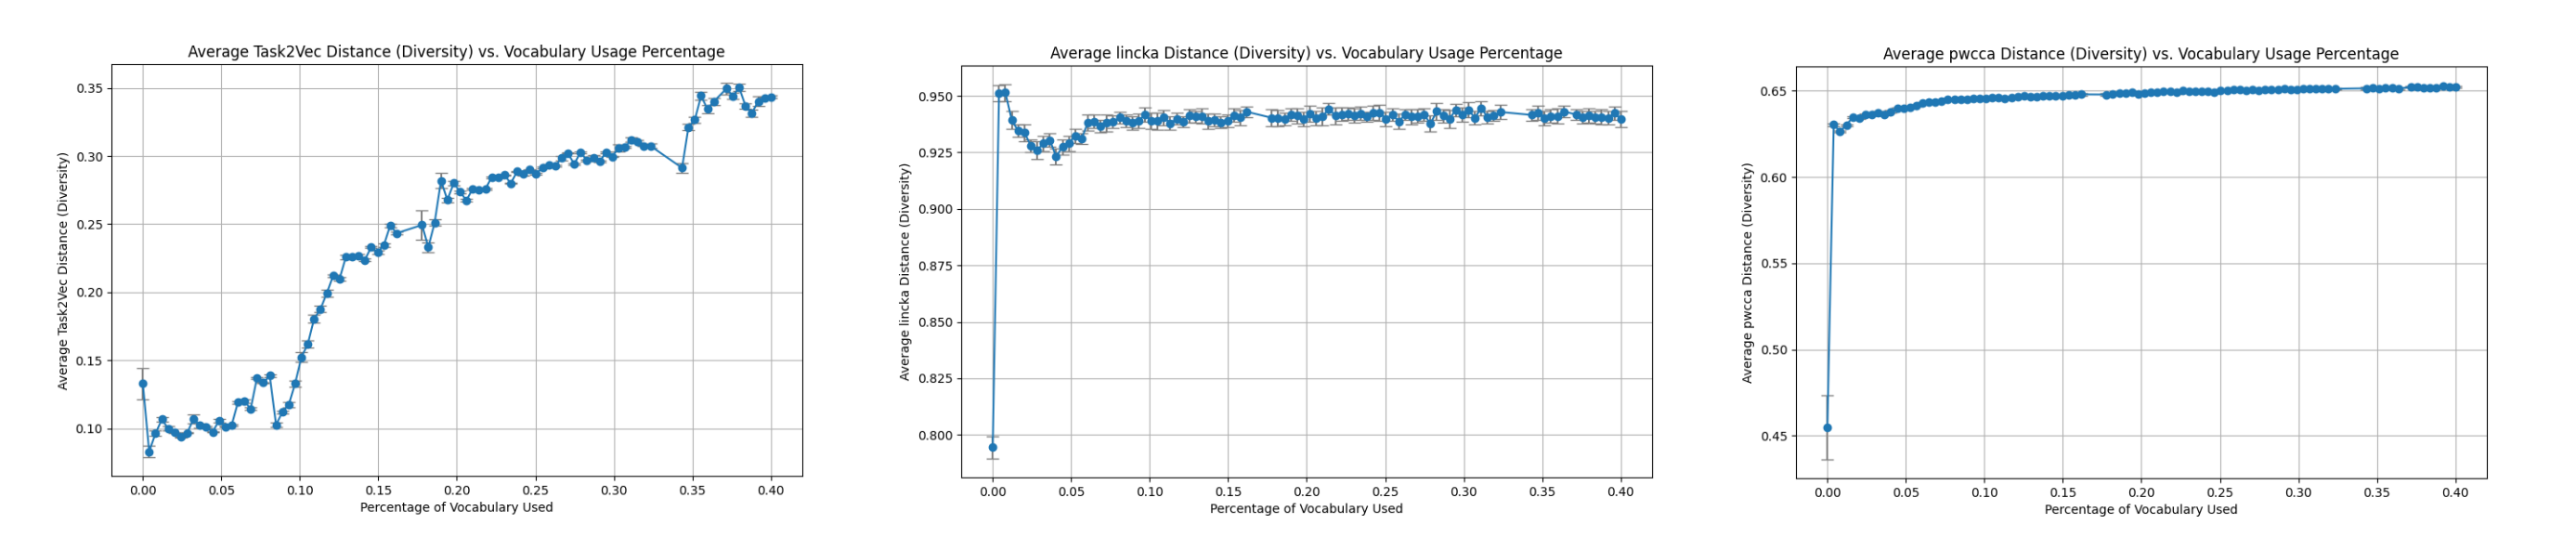
\includegraphics[width=1.0\linewidth]{plots/div_acts_vs_task2vec_92.png}
    % \vspace{5mm} % Adjust the 5mm as needed for your layout
    % 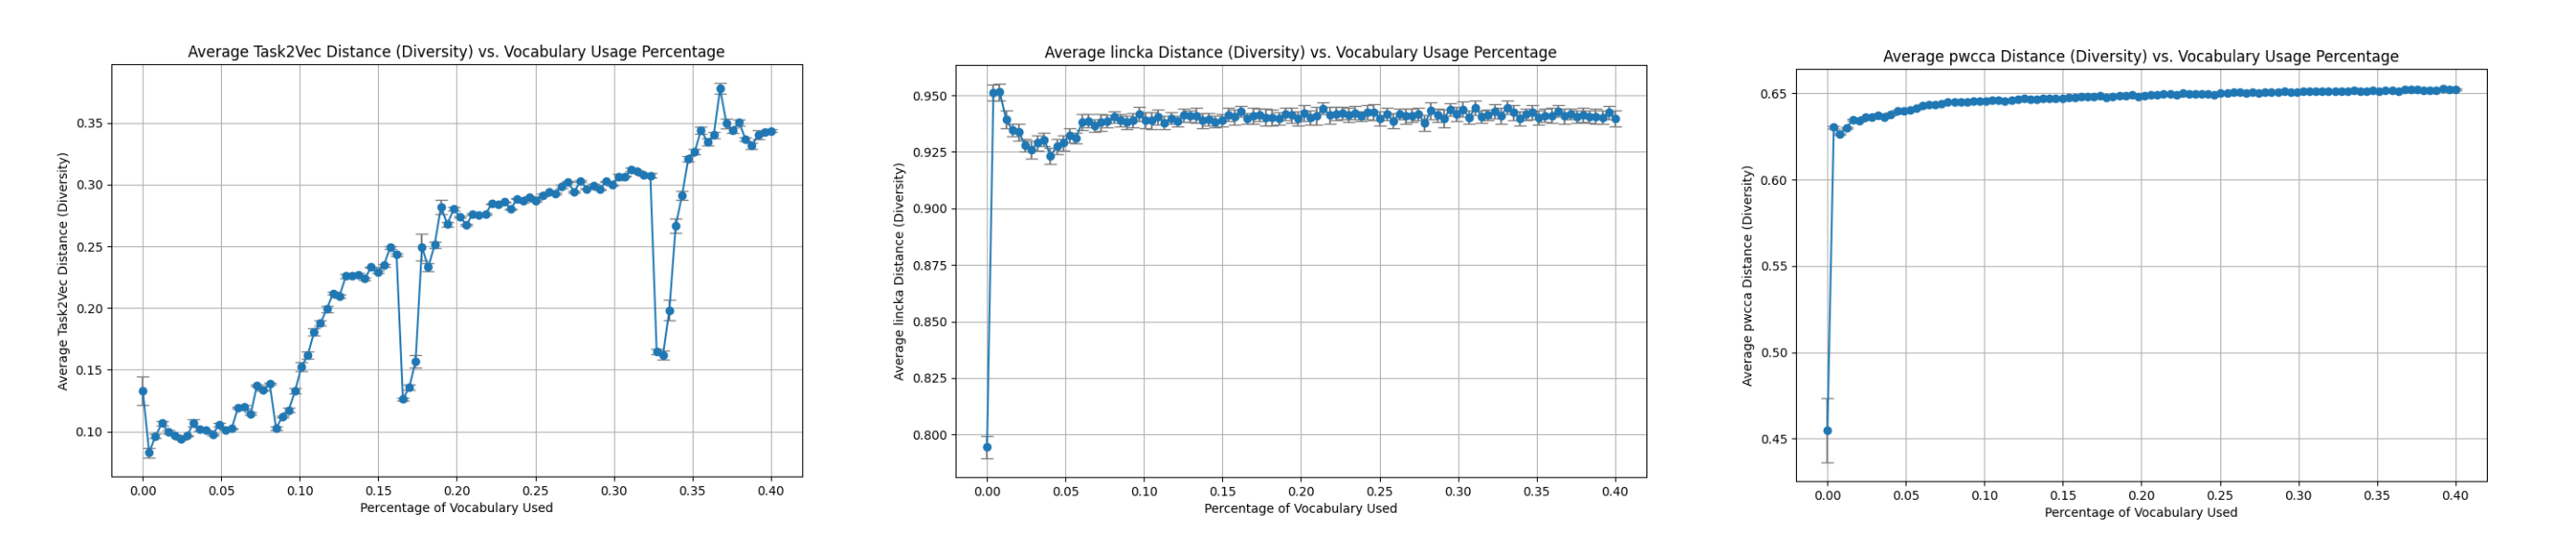
\includegraphics[width=1.0\linewidth]{plots/div_acts_vs_task2vec_100.png}
    
\includegraphics[width=1.0\linewidth]{plots/div_acts_vs_task2vec_wandb_smoothed.png}
    \caption{\textbf{Shows the resolution power deficit in activation-based diversity approaches compared to Task2Vec Diversity.} 
    We plot the diversity on the y-axis against percentage of the vocabulary used on the x-axis. 
    Varying the vocabulary varies the diversity of a data set because the smaller the vocabulary, the more homogenous the sequence of text will be. 
    For example, vocabulary size 1 gives the same sequence while $|V|$ allows for $|V|^T$ possible sequences.
    After only $8.09\%$ of the x-axis, the activation based diversity increased to it's maximum values and remains approximately constant within 95\%-confidence intervals, while Task2Vec diversity increases smoothly. 
    To make the patterns clearer, we smoothed out the top three plots by removing outliers and used a smoothing value of 0.79 in the bottom three plots. 
    The outlier plots can be recovered by observing at the light blue line in the bottom three plots. 
    We conjecture that the outlier were caused by the small number of batches we used (30). 
    }
    \label{fig:div_acts_vs_task2vec}
\end{figure*}

\subsection{Token Based Definitions of Diversity are Brittle to Paraphrasings}
One can also consider formalizations of diversity based on token distributions in a batch (or data set). 
We did not use this because previous work has already demonstrated its limitation as data representations for train-test data contamination detection \citep{contamination}. 
This is highly related to our work because contamination detection requires good data representations for detecting differences in text. 
In particular, they say: ``these contamination definitions primarily revolve around n-gram or token overlaps, which only target direct duplications present in both training and evaluation datasets and might provide both high false positive rate (since many semantically different texts have overlaps) and false negative rate (since simple paraphrasing can evade detection)".
To make it more concrete, consider an example. 
Consider the sentences ``The great paper" and ``the fantastic paper". 
These would be binned to entirely different locations in a histogram, while the difference in the sentence is varying much more smoothly. 
Therefore, token based representation of data are brittle to simple paraphrasing and as our example shows result in overly ``harsh" metrics---similar to previous work that criticizes harsh metrics for LLM evaluation \citep{mirage}. 
In addition, previous work has shown that importance weights of data like text are statistically intractable to estimate without sufficient additional structure \citep{dsir, Bengtsson_2008, GelmanMeng2004, SnyderEtAl2008}. 
For example, the histograms of different types of text end up being sparse, even with hashing e.g., consider 50k (GPT2), 30K (LLaMA2) or 10K (DSIR) feature vectors. 
We conjecture that if these representations were robust, the transformer architecture \citep{vaswani2017attention} wouldn't have emerged as the successful architecture that it is today (2024). 
% TODO: do token based experiments for semantics clustering.

\subsection{Discussion on Model Agnostics Formalizations of Data Diversity}\label{kolmogorov_fisher_relation}
\textbf{Theoretical Relation of FIM (Model) and Kolmogorov (Model Agnostic) based metric: } 
Theory can be important to have a better understanding of the world. 
Therefore, theoreticians might be interested in diversity definitions that are model agnostic, since, they might be interested in the inherit diversity of the data or task. 
We emphasize that Task2Vec was derived with such considerations in mind: 
``The FIM is also related to the (Kolmogorov) complexity of a task, a property that can be used to define a computable metric of the learning distance between tasks" \citep{task2vec}.
More precisely \citep{AchilleMbengSoatto2018} showed that the training dynamics of a deep network minimizing a loss function can be viewed as approximately optimizing an upper bound on the Kolmogorov Structure Function (KSF) of the learning task. 
This connection arises because the loss function incorporates a complexity term measured by the Fisher Information Matrix of the network weights. 
Therefore, Fisher information provides a computable way to relate the geometry of the loss landscape to notions of task complexity linked to Kolmogorov complexity. 
% However, explicit relationships quantifying how distances based on Fisher information matrices correlate with true Kolmogorov complexity are not provided.
Therefore, Task2Vec (via FIM) was derived with Kolmogorov Complexity in mind. 
In Summary, the relationship between Fisher Information Matrix (FIM) and Kolmogorov Complexity, as discussed in Achille's works \citep{task2vec, AchilleMbengSoatto2018, achille2019dynamics, AchillePaoliniMbengSoatto2021}, suggests that FIM can serve as an upper bound for Kolmogorov Complexity in the context of learning tasks. 
Specifically, the FIM captures the sensitivity of the learning model to its parameters, reflecting the amount of information about the data that the model encodes. 
This sensitivity can indirectly bound the Kolmogorov Complexity by quantifying the model's complexity and its capacity to learn from data, thus offering a bridge between empirical measures of complexity (FIM) and theoretical ones (Kolmogorov Complexity).
However, explicit relationships quantifying how distances based on Fisher information matrices correlate with true Kolmogorov complexity are not provided.

\textbf{Remarks on approximations to Kolmogorov: }
The central way we control for our results to be model agnostic in practice is by fixing the model. 
This means that the data is the only thing being varied, and the features being used for any diversity of computations are consistent. 
Since, Kolmogorov Complexity in uncomputable we conjecture this is approximately optimal---given that it's essential in practice to have a way to represent the data. 

% TODO: https://alexachi.github.io/files/achilleMS18dynamics.pdf
% We bring to bear tools from diverse fields, from Kolmogorov Complexity
% to quantum physics, to enable defining and computing sensible notions of distance that correlate with
% ease of transfer learning. In the process, we discover interesting connections between seemingly
% disparate concepts: The first is between the notion of task reachability, which we introduce, and the
% Kolmogorov Structure Function. This in turn is related to information-theoretic treatments of deep
% learning that have been recently developed [4].

% TODO: finish perhaps connect Fisher and Kolmogorov: https://www.overleaf.com/project/616da56221637be4a0b6b5e0
% \subsection{Distance of a task according to Task2Vec and related work}
% In this section we will give our review of related work by \cite{Achille_dist_tasks, task2vec} to define distances between task, complexity, embeddings of tasks and related concepts.
% \subsubsection{Static Distance between tasks}
% To define the static distance between tasks \cite{Achille_dist_tasks} first define the complexity of a task then define the static distance using the complexity of a task.
% \textbf{Task:} \cite{Achille_dist_tasks} define a task $\tau$ as the r.v. $y$ one is trying to infer given $x$ or the representing data set for the random variables with a loss function.
% We also consider that definition and the usual k-shot, n-way few-shot learning definitions of tasks.
% \textbf{Ideal Complexity of a task:} The complexity $C(\tau)$ of a task $\tau$ should be a metric that captures the difficulty/complexity (e. best length, optimal encoding length) to approximately describe a task given a model $m$.
% Recall that the Kolmogorov complexity $k(x)$ does this for bit strings $x$ - where $k(x)$ is the shortest program (assuming a fixed programming language) to output $x$ and halt.
% The more difficult and complex a task the more bits the best (e.g. smallest) description will need to encoding the task.
% Building from this idea one can define the complexity of a task as the minimum length (i.e. difficulty) to describe a model $M$ that approximately describes (e.g. fits, compresses) a task $\tau$ with loss at most $l$ loss:
% \begin{equation}
%     S_{\tau}(l) = \min_{m \in \mathcal M : L_\tau(m) < l}{ k(m) }
% \end{equation}
% where $m$ is the model, $\mathcal M$ is the model class, $k$ is the kolmogorov complexity, $L_\tau(m)$ is the loss of model $m$ on task $\tau$ (e.g. cross-entropy loss) and $l$ is the target loss.
% This function is also called the Kolmogrov Structure Function \cite{Achille_dist_tasks}.
% Using standard optimization techniques the complexity of a task $\tau$ can be re-written in Lagrangian form:
% \begin{equation}
%    C_{\beta}(\tau; m)  = L_{\tau}(m) + \beta k(m)
% \end{equation}
% for a certain $\beta$ this corresponds to a certain complexity and loss value $l_{\beta}$.
% Intuitively, this measure the cost of encoding $\tau$ (or the data set) using model $m$ when the cost the model $k(m)$ is discounted by a factor of $\beta$ \cite{Achille_dist_tasks}.
% Thus \textbf{the complexity of a task} $\tau$ (or data set) with level $\beta$ is:
% \begin{equation}
%    C_{\beta}(\tau) = \min_{m \in \mathcal M} C_{\beta}(\tau; m)  = \min_{m \in \mathcal M} L_{\tau}(m) + \beta k(m)
% \end{equation}
% which measure the complexity at level $\beta$ to describe task $\tau$ with the best model $m$ in the model class $\mathcal M$ or the difficulty of encoding task $\tau$ using the best model in model class $\mathcal M$ at level $\beta$.
% \textbf{Approximation of the Complexity of a task:}
% TODO lower bound
% \textbf{Static Distance:}
% TODO.
% \subsubsection{Dynamic Distance between tasks}

\section{LLM Pre-training Datasets}
\label{appendix:datasets}
Since LLMs are often trained on internal, non-public datasets\footnote{For instance, Gopher was trained on Google's internal dataset MassiveText.}, we used publicly available language datasets from the same sources as LLM pre-training data:

\textbf{C4}, a 305GB cleaned version of Common Crawl's web crawl corpus in English \cite{C4}. Sequences in C4 were extracted from the web via de-duplication methods and heuristics to remove boiler-plate and gibberish.

\textbf{WikiText-103}, a 500MB collection of over 100 million tokens extracted from the set of verified Good and Featured articles on Wikipedia \cite{wikitext}. 

\textbf{The Pile}, a 825 GiB open-source English-text corpus for language modeling that combines 22 smaller, high-quality datasets from diverse sources \cite{thepile}. These sources include Pile-CC (Common Crawl), PubMed Abstracts, Books3, OpenWebText2, ArXiv, and GitHub. 

\textbf{SlimPajama},
an open-source reproduction of the LLaMA v1 dataset with extensively deduplication. It incorporates data from CommonCrawl (CC), C4, GitHub, Books, ArXiv, Wikipedia, and StackExchange, totaling 627 billion tokens \cite{cerebras2023slimpajama}.
% RedPajama is an open-source implementation of the LLaMa v1 dataset, incorporating data from CommonCrawl (CC), C4, GitHub, Books, ArXiv, Wikipedia, and StackExchange, totaling 1.2 trillion tokens.
% Slim Pajamas is extensively deduplicate RedPajama. % to produce a dataset with higher information density that achieves higher accuracy with same compute. 
% This means when using SlimPajama, you can achieve higher accuracy with the same compute budget when compared to other datasets.

For instance, GPT-3 was trained on a filtered Common Crawl dataset and Wikipedia \cite{gpt3}, which are represented by C4 and WikiText-103. It was also trained on WebText2 and Books, which are sub-datasets of The Pile.

We also evaluate the diversity coefficient of the following six sub-datasets of The Pile:

\textbf{Pile-CC}, a 227 GiB preprocessed version of Common Crawl's web crawl corpus \cite{thepile}. While both Pile-CC and C4 are sourced from Common Crawl, Pile-CC was preprocessed from Web Archive files, which are raw HTTP responses and page HTML, whereas C4 was preprocessed from WET files, which consist of plaintext. Nonetheless, we expect that both datasets are non-mutually-exclusive.

\textbf{HackerNews}, a 4 GiB scraped and parsed dataset of comment trees from Hacker News, a social news website that aggregates article links \cite{thepile}. Articles are generally focused on topics in computer science and entrepreneurship.

\textbf{NIH ExPorter}, a 1.9 GiB dataset of NIH Grant abstracts for awarded applications from 1985-present hosted on the ExPORTER initiative \cite{thepile}.

\textbf{PubMed Abstracts}, a 19 GiB dataset of abstracts from 30 million publications in PubMed \cite{thepile}.

\textbf{USPTO Backgrounds}, a 23 GiB dataset of background sections from patents granted by the United States Patent and Trademark Office (USPTO) \cite{thepile}.

\textbf{OpenWebText2}, a 38 GiB dataset based on data extracted from Reddit posts, deduplicated, and filtered for English content using FastText. 
% Web pages were pulled using the newspaper python package, and near-duplicates were identified and removed using local-sensitivity hashing (LSH). 
% Only documents with a unique content similarity of less than 0.5 and more than 128 tokens were retained. 
Strict filtering with local-sensitive hashing (LSH) was done and only unique content with similarity of less than 0.5 was used. % and more than 128 tokens were retained.
The finalized dataset comprises 38 GiB. % from 8,013,769 documents. 
% Annotations: None present in the dataset.
% Used to train GPT2.

% These five sub-datasets were selected for streaming support on HuggingFace, and for relatively efficient streaming time. 
%See Appendix \ref{appendix:experiment_details} for dataset preprocessing and experimental details.
 

\section{Further Justification and Explanation of Cross Diversity}
\label{appendix:cross_div_justification}

We include the notion of the cross diversity coefficient as it also leverages the ability of distance between Task2Vec embeddings to capture important properties of the data, and allows one to more clearly assess similarity/diversity \textit{between} datasets (hence the term \textit{cross} diversity), as opposed similarity/diversity \textit{within} datasets (the focus of the ``normal" diversity coefficient). Thus, when information on clearly defined sub-datasets is available, one can use cross-diversity to more specifically determine the diversity of the concatenation of the given datasets (to form the total/overall dataset). Thus, the cross diversity coefficient provides us the opportunity to more robustly characterize methods of defining data diversity by offering a different perspective on combined datasets from the diversity coefficient. Note that in the case $D_1 = D_2$, i.e. one is calculating the cross diversity of a single dataset (with itself), cross diversity becomes equivalent to diversity.

\section{Task2Vec Diversity Coefficient Correlates with Ground Truth Diversity}
\label{appendix:ground_truth_div}
\begin{figure*}[h]
    \centering 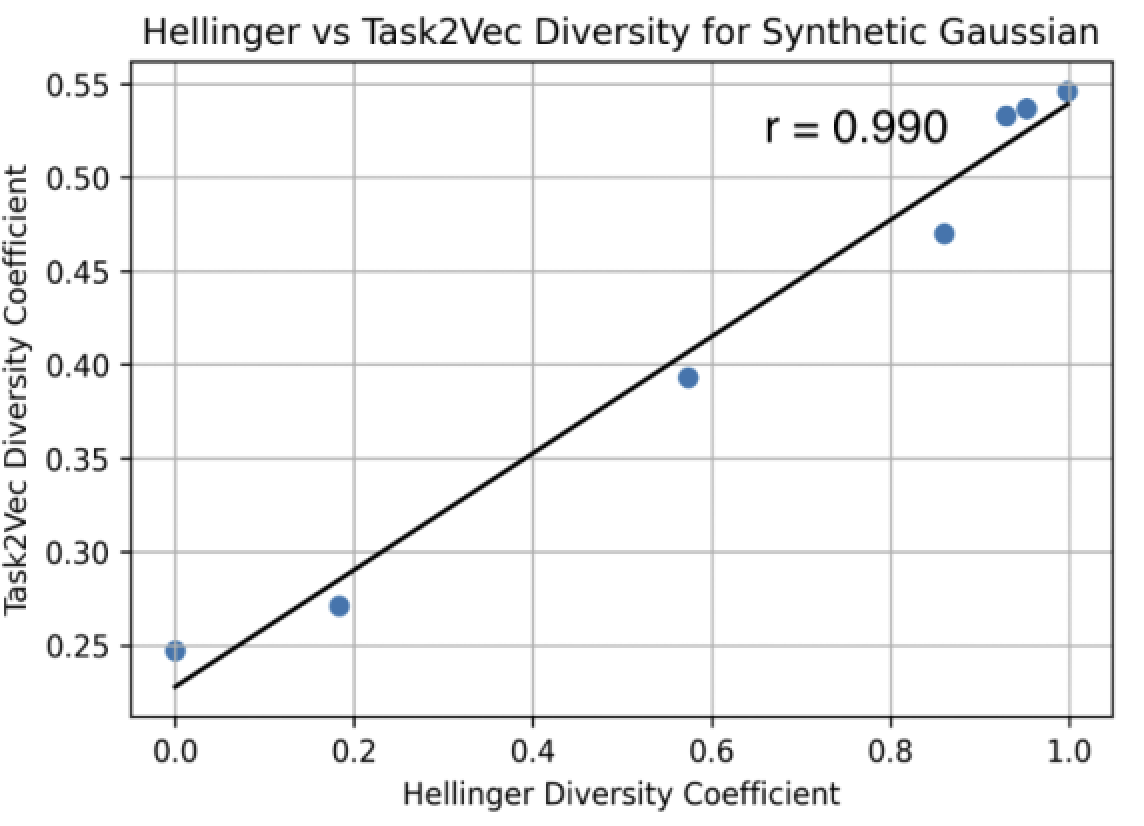
\includegraphics[width=0.5\columnwidth]{plots/truth_vs_task2vec.png}
    \caption{\textbf{Task2Vec diversity coefficient correlates with ground truth diversity for synthetic Gaussian benchmark.} Source: \cite{diversity}}
\end{figure*}

As shown in \cite{diversity}, when the ground truth diversity is available for a synthetic Gaussian benchmark, the Task2Vec diversity coefficient correlates with the ground truth diversity. These results provide confidence in the Task2Vec diversity coefficient as diversity metric.

% \section{Pipeline for Diversity Coefficient Computation of Natural Language Datasets}
% \label{appendix:pipeline}
% \begin{figure}
%     \begin{center}
%         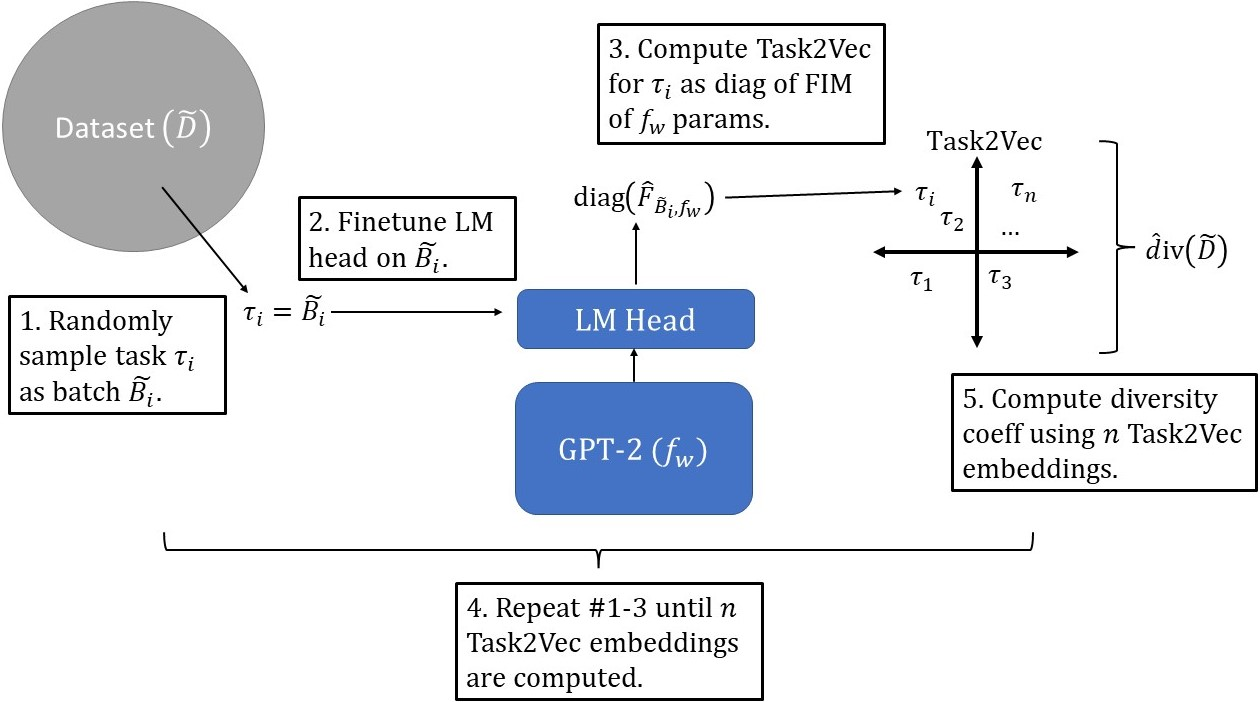
\includegraphics[width=0.7\columnwidth]{plots/diversity_project_figure_spreadout_cropped.jpg}
%     \end{center}
%   \caption{\textbf{A depiction of a pipeline to compute the Task2Vec diversity coefficient for a natural language dataset.}}
%   \label{fig:pipeline}
% \end{figure}

Figure \ref{fig:div_pipeline} shows our pipeline for computing the diversity coefficient of large scale, natural language datasets. See section \ref{body:div_coeff_natural_lang} for more details on our method.

\section{Higher Formal Diversity of the Training Data Set Causes Higher Test Performance}
Table \ref{tab:div_vs_ppl} demonstrates the causal relationship between pre-training data diversity and downstream evaluation performance on a diverse target domain. 

\subsection{Higher Formal Diversity of the Training Data Set Causes Higher Test Performance: GPT2 Results}

% NEW RESULTS (post Feb/1)
\begin{table}[h!]
    \centering
    \caption{\textbf{The table illustrates that as the diversity coefficient of training data increases, the cross-entropy loss (CE) decreases on diverse tasks, implying that training on higher diversity data improves evaluation performance on diverse tasks.} 
    Each model is trained for the same number of tokens (1.31 B tokens total), 
    all models have 51.5 M parameters, and all use a GPT-2-based architecture; all other hyperparameters are identical and controlled for.
    We evaluate on Pile-CC (Pile Common Crawl) and OpenWebText2 since those datasets align with intuitively diverse datasets, which we verify with the computed diversity values shown.
    }
    \vspace{10pt}
    \begin{tabular}{lccc}
        \toprule
        Training Data Set & OpenWebText2 (\textbf{div 0.222}) \\
        \midrule
        USPTO (\textbf{div 0.158}) & 6.4414 \\
        PubMed (\textbf{div 0.168})  & 6.4204 \\
        USPTO + PubMed (\textbf{div 0.195}) & \textbf{6.1815} \\
        \bottomrule
    \end{tabular}
    \label{tab:div_vs_ppl}
\end{table}

% % NEW RESULTS (post 11/20)
% \begin{table}[h!]
%     \centering
%     \caption{\textbf{The table illustrates that as the diversity coefficient of training data increases, the cross-entropy loss (CE) decreases on diverse tasks, implying that training on higher diversity data improves evaluation performance on diverse tasks.} 
%     Each model is trained for the same number of tokens (1.31 B tokens total), 
%     all models have 51.5 M parameters, and all use a GPT-2-based architecture; all other hyperparameters are identical and controlled for.
%     We evaluate on Pile-CC (Pile Common Crawl) and OpenWebText2 since those datasets align with intuitively diverse datasets, which we verify with the computed diversity values shown.
%     }
%     \begin{tabular}{lccc}
%         \toprule
%         Training Data Set & Pile-CC (\textbf{div 0.250}) & OpenWebText2 (\textbf{div 0.222}) \\
%         \midrule
%         USPTO (\textbf{div 0.158}) & 5.9988 & 6.4414 \\
%         PubMed (\textbf{div 0.168})  & 6.1412 & 6.4204 \\
%         USPTO + PubMed (\textbf{div 0.195}) & \textbf{5.7954} & \textbf{6.1815} \\
%         \bottomrule
%     \end{tabular}
%     \label{tab:div_vs_ppl}
% \end{table}

% \begin{table*}[h]
% \centering
% \begin{tabularx}{1\textwidth}{lXXXXX} \hline 
% Archetype& \# Tokens & Dataset  & OpenWebText2  & C4 & WikiText-2 \\ \hline 
% GPT-2-51M & 550M & USPTO  & 680.275 & 337.6114 &  621.6839 \\
% - & - & PubMed & 577.4589  & 383.4001   & 579.2974\\
% - & - & USPTO+PubMed & 511.3447  & 281.1059 & 461.6712 \\ \hline
% GPT-2-51M & 1.31B & USPTO &    652.1721 & 363.4589 & 633.3967 \\ 
% - & - & PubMed &      610.6643  & 299.0154 & 621.2794 \\
% - & - & USPTO+PubMed &   496.4988  & 138.7324  & 452.7013 \\ \hline
% GPT-2-345M &  2.23B & USPTO & 511.3447 & 219.4235  & 387.5332  \\ 
% - & - & PubMed & 304.5564   & 160.4508 & 224.0043  \\
% - & - &  USPTO+PubMed & 251.2429   & 138.7324 & 166.1276 \\ \hline
% GPT-2-810M &  1.97B & USPTO & 5.59 & 5.00  & TODO/NA  \\ 
% - & - & PubMed & 5.48   & 4.95 & TODO/NA  \\
% - & - &  USPTO+PubMed & 5.40   & 4.82 & TODO/NA \\ \hline
% \end{tabularx}
% \caption{Calculated Perplexity on Various High Diversity Datasets}
% \label{table:openwebtext}
% \end{table*}

\subsection{Higher Formal Diversity of the Training Data Set Causes Higher Test Performance: All Results}
Table \ref{tab:div_vs_ce_val} demonstrates how the cross-entropy of the validation loss decreases as the diversity of the pre-training data set increases. 
All tokens were fixed. 
The table includes LLaMAv2 7B results trained from scratch.

\begin{table*}[h]
\caption{\textbf{Cross-entropy of the validation loss decreases as the diversity of the pre-training data set increases}. 
We report the test cross-entropy (no parenthesis) and the corresponding perplexity (in parentheses) on the validation set of C4, OpenWebText2).
The diversity of the evaluation data sets, C4 and OpenWebText2 is 0.222, 0.237 respectively. 
The pre-train diversity of USPTO, PubMed, USPTO+PubMed is 0.158, 0.168, and 0.195 respectively.
All evaluations were on the full validation set except for the ones denoted as [8B] which used a batch size of size 8 due to runs crashing due to random hardware failure when running such large evaluations. 
C4's validation set has 365K examples. 
OpenWebText2 had 33.4k examples. 
We explicitly avoided evaluating on the pile to minimize cofounders on our experiments, e.g., that the good performance might be due to data contamination. 
We also evaluated on two data sets for the same reasons and to increase robustness of our observations. Table entries are continued in Table \ref{tab:div_vs_ce_val_cont}.
}
\vspace{10pt}
\centering
\begin{tabularx}{1\textwidth}{lXXXX} 
\bottomrule 
Architecture & \# Tokens (Seq Len) & Train Dataset  & OWT2 (\textbf{div 0.222})  & C4 (\textbf{0.237}) \\
\bottomrule 

LLaMA2-7B (Scratch, run1) & 6.36M (1024 L) & USPTO  & 7.99 (2959.1) & 7.22 (1372.9) \\ % https://wandb.ai/brando/beyond-scale/runs/022np2zn/logs?workspace=user-brando
- & - & PubMed & 8.038 (3097.6) & 7.26 (1424.3) \\ % https://wandb.ai/brando/beyond-scale/runs/mqod4h24/logs?workspace=user-brando
- & - & USPTO + PubMed & 7.67 (2144.2) & 6.90 (999.6) \\ % https://wandb.ai/brando/beyond-scale/runs/6wsejybj/logs?workspace=user-brando
\hline

LLaMA2-7B (Scratch, run2) & 6.36M (1024 L) & USPTO  & 8.048 (3127.0) & 7.23 (1385.5) \\ % https://wandb.ai/brando/beyond-scale/runs/i5qbnmcs/logs?workspace=user-brando
- & - & PubMed & 7.82 (2496.0) & 7.11 (1225.0) \\ % https://wandb.ai/brando/beyond-scale/runs/zqv29bjc/logs?workspace=user-brando
- & - & USPTO + PubMed & 7.83 (2154.6) & 7.08 (1189.5) \\ %% https://wandb.ai/brando/beyond-scale/runs/3o05mvz6/logs?workspace=user-brando
\hline

LLaMA2-7B (Scratch, run3) & 6.36M (1024 L) & USPTO  & 7.90 (2706.2) & 7.10 (1216.5) \\ % https://wandb.ai/brando/beyond-scale/runs/ilha1tub/logs?workspace=user-brando
- & - & PubMed & 7.82 (2513.4) & 7.06 (1172.8) \\ % https://wandb.ai/brando/beyond-scale/runs/1wo1n4ek/logs?workspace=user-brando
- & - & USPTO + PubMed & 7.84 (2548.8) & 7.02 (1126.7) \\ % https://wandb.ai/brando/beyond-scale/runs/s9ou7l1n/logs?workspace=user-brando
\hline

LLaMA2-7B (Scratch, run4) & 6.36M (1024 L) & USPTO  & 7.94 (2826.9) & 7.14 (1267.2) \\ % https://wandb.ai/brando/beyond-scale/runs/hxhn2wng/logs?workspace=user-brando
- & - & PubMed & 7.78 (2396.3) & 7.01 (1112.6) \\ % https://wandb.ai/brando/beyond-scale/runs/1s5usylp/logs?workspace=user-brando
- & - & USPTO + PubMed & 7.67 (2154.6) & 6.93 (1030.4) \\ % owt2 eval: https://wandb.ai/brando/beyond-scale/runs/q54jr2nq/logs?workspace=user-brando    c4 eval: https://wandb.ai/brando/beyond-scale/runs/ffi89h7s/logs?workspace=user-brando
\hline



\bottomrule
\end{tabularx}
\label{tab:div_vs_ce_val}

\end{table*}






\begin{table*}[h]
\caption{\textbf{Continuation of Table \ref{tab:div_vs_ce_val}.}}
\vspace{10pt}
\centering
\begin{tabularx}{1\textwidth}{lXXXX} 
\bottomrule 
Architecture & \# Tokens (Seq Len) & Train Dataset  & OWT2 (\textbf{div 0.222})  & C4 (\textbf{0.237}) \\
\bottomrule 
LLaMA2-7B (Scratch, run5) & 25.4M (1024 L) & USPTO  & 8.10 (3302.1) & 7.31 (1497.0) \\ % https://wandb.ai/brando/beyond-scale/runs/3cgbdsb2/logs?workspace=user-brando
- & - & PubMed & 7.70 (2217.1) & 6.97 (1067.7) \\ % https://wandb.ai/brando/beyond-scale/runs/ocndcuy2/logs?workspace=user-brando
- & - & USPTO + PubMed & 7.65 (2108.8) & 6.87 (966.8) \\ % https://wandb.ai/brando/beyond-scale/runs/nlknrs4k/logs?workspace=user-brando
\hline
LLaMA2-7B (Scratch, run6) & 25.4M  (1024 L) & USPTO  & 8.00 (2999.6) & 7.23 (1385.0) \\ % https://wandb.ai/brando/beyond-scale/runs/crxpf5bg/logs?workspace=user-brando
- & - & PubMed & 7.82 (2511.3) & 7.09 (1205.2) \\ % https://wandb.ai/brando/beyond-scale/runs/fj5xd2kj?workspace=user-brando
- & - & USPTO + PubMed & 7.76 (2351.7) & 7.02 (1120.1) \\ % https://wandb.ai/brando/beyond-scale/runs/2dy8rrcc/logs?workspace=user-brando
\hline

LLaMA2-7B (Scratch, run7) & 25.4M (4096 L) & USPTO  & 7.54 (11881.9) & 6.69 (809.5) \\ % https://wandb.ai/brando/beyond-scale/runs/ghjkc8tc/logs?workspace=user-brando
- & - & PubMed & 7.16 (1293.7) & 6.45 (634.1) \\ % https://wandb.ai/brando/beyond-scale/runs/7jqujyv1/logs?workspace=user-brando
- & - & USPTO + PubMed & 7.26 (1425.0) & 6.36 (578.2) \\ % https://wandb.ai/brando/beyond-scale/runs/ad2f1yew/logs?workspace=user-brando
\hline

% LLaMA2-7B (Scratch, run8) & 25.46M (4096L) & USPTO  & 7.54 & 6.69 \\ % https://wandb.ai/brando/beyond-scale/runs/ghjkc8tc/overview?workspace=user-brando
% - & 25.46M (4096L) & PubMed & 7.16 & c4 eval failed \\ % https://wandb.ai/brando/beyond-scale/runs/7jqujyv1/logs?workspace=user-brando
% - & 25.46M (4096L) & USPTO+PubMed & 7.26 & 6.36 \\ % https://wandb.ai/brando/beyond-scale/runs/ad2f1yew/logs?workspace=user-brando
% \hline

GPT2-51M & 328M (1024L) & USPTO  & 6.91 (998.6) & 6.34 (568.3) \\ 
- & - & PubMed & 6.82 (912.5) & 6.30 (543.2) \\ 
- & - & USPTO + PubMed & 6.89 (984.3) & 6.23 (505.7) \\
\hline
GPT2-51M & 550M (1024L) & USPTO  & 6.47 (646.6) & 5.82 (338.5) \\ 
- & - & PubMed & 6.36 (575.7) & 5.85 (348.1) \\ 
- & - & USPTO + PubMed & 6.20 (491.0) & 5.63 (279.7) \\
\hline
GPT2-117M & 2.2B (1024L) & USPTO  & 5.86 (351.5) & 5.29 (197.8) \\ 
- & - & PubMed & 5.82 (337.7) & 5.30 (200.0) \\ 
- & - & USPTO + PubMed & 5.71 (301.4) & 5.15 (171.7) \\ 
\hline
GPT2-204M & 1.31B (1024 L) & USPTO  & 6.16 (473.4) & 5.40 (221.4) \\ 
- & - & PubMed & 5.75 (314.2) & 5.25 (190.6) \\ 
- & - & USPTO + PubMed & 5.60 (270.4) & 5.05 (156.0) \\ 
% \hline
% GPT2-345M & 2.2B (1024L) & USPTO  & 5.67 (289.4) & 5.06 (158.1) \\ 
% - & - & PubMed & 5.54 (254.9) & 5.04 (155.1) \\ 
% - & - & USPTO+PubMed & 5.46 (234.0) & 4.90 (134.7) \\
% \hline
% GPT2-51M & 1.31B (1024L) & USPTO  & 6.44 (627.3) & 5.90 (363.3) \\ 
% - & - & PubMed & 6.42 (614.27) & 5.92 (372.5) \\ 
% - & - & USPTO+PubMed & 6.15 (469.09) & 5.68 (291.69) \\
% \hline
% GPT2-810M & 2B (1024 L) & USPTO  & 5.59 (267.7) & 5.00 (148.4) \\ 
% - & - & PubMed & 5.48 (239.8) & 4.95 (141.2) \\ 
% - & - & USPTO+PubMed & 5.40 (221.4) & 4.82 (124.0)\\
% \hline
% GPT2-1.5B & 180M (1024L) & USPTO  & 7.28 (1454.0) & 6.12 (454.13) \\ 
% - & - & PubMed & 6.40 (599.5) & 5.80 (328.7) \\ 
% - & - & USPTO+PubMed & 6.45 (630.2) & 5.68 (294.4) \\
% \hline

\bottomrule
\end{tabularx}
\label{tab:div_vs_ce_val_cont}

\end{table*}

% \section{Role of Data Alignment Coefficient on Test Performance}
% Given a distance function for a batch of data (or task) one can also measure how aligned or similar two data sets.
% One can do this by computing the cross diversity between batches/tasks of data and then subtract one from it. 
% Therefore, we propose one minus the cross diversity coefficient as the definition of the alignment coefficient:
% \begin{equation*}
% \begin{aligned}
%     \textrm{$\hat{align}$}(D_1, D_2) =
%     1 -
%     \mathbb{E}_{B_1 \sim D_1, B_2 \sim D_2} 
%      % \left[ 
%      d( \vec{f}_{B_1}, \vec{f}_{B_2} )
%      % \right]
% \end{aligned}
% \end{equation*}
% We choose this method since:
% \begin{enumerate}
%     \item It is simple to define given the definition of cross diversity proposed in this paper.
%     \item It provides simple confidence interval to compute given that it's an expectation---in contrast to using a large batch of data and the cosine distance of two Task2vec batch/task embeddings.
% \end{enumerate}
% Figure \ref{fig:align_corr} demonstrates that there is a moderate-strong relationship between the alignment coefficient (between pre-train data and evaluation data) and model performance (cross entropy loss) on various evaluation datasets ($r^2 = 0.80, r=-0.89$).
% The raw alignment values with 95\% confidence are reported at \ref{fig:align_table} and, as expected, when datasets share similarities in topic and structure, the alignment coefficient is higher (see caption of table).
% In addition, Figure \ref{fig:outputs_are_good_despite_high_loss} shows that despite the arguably high loss, the models are pre-trained enough to grasp important aspects of sentence syntax and structure of their respective dataset.

%\textbf{The data alignment coefficient demonstrates a solid relationship to model performance (cross entropy loss) on various evaluation datasets ($r^2 = 0.80, r=0.89$)}. 
    %The data alignment coefficient is computed between a model's pre-training dataset (PubMed Abs., USPTO, or PubMed Abs. + USPTO) and a single evaluation dataset (represented by a unique color).
%%%%%%%%%%%%%%%%%%%%%%%%
% \begin{figure}
%     \centering
%     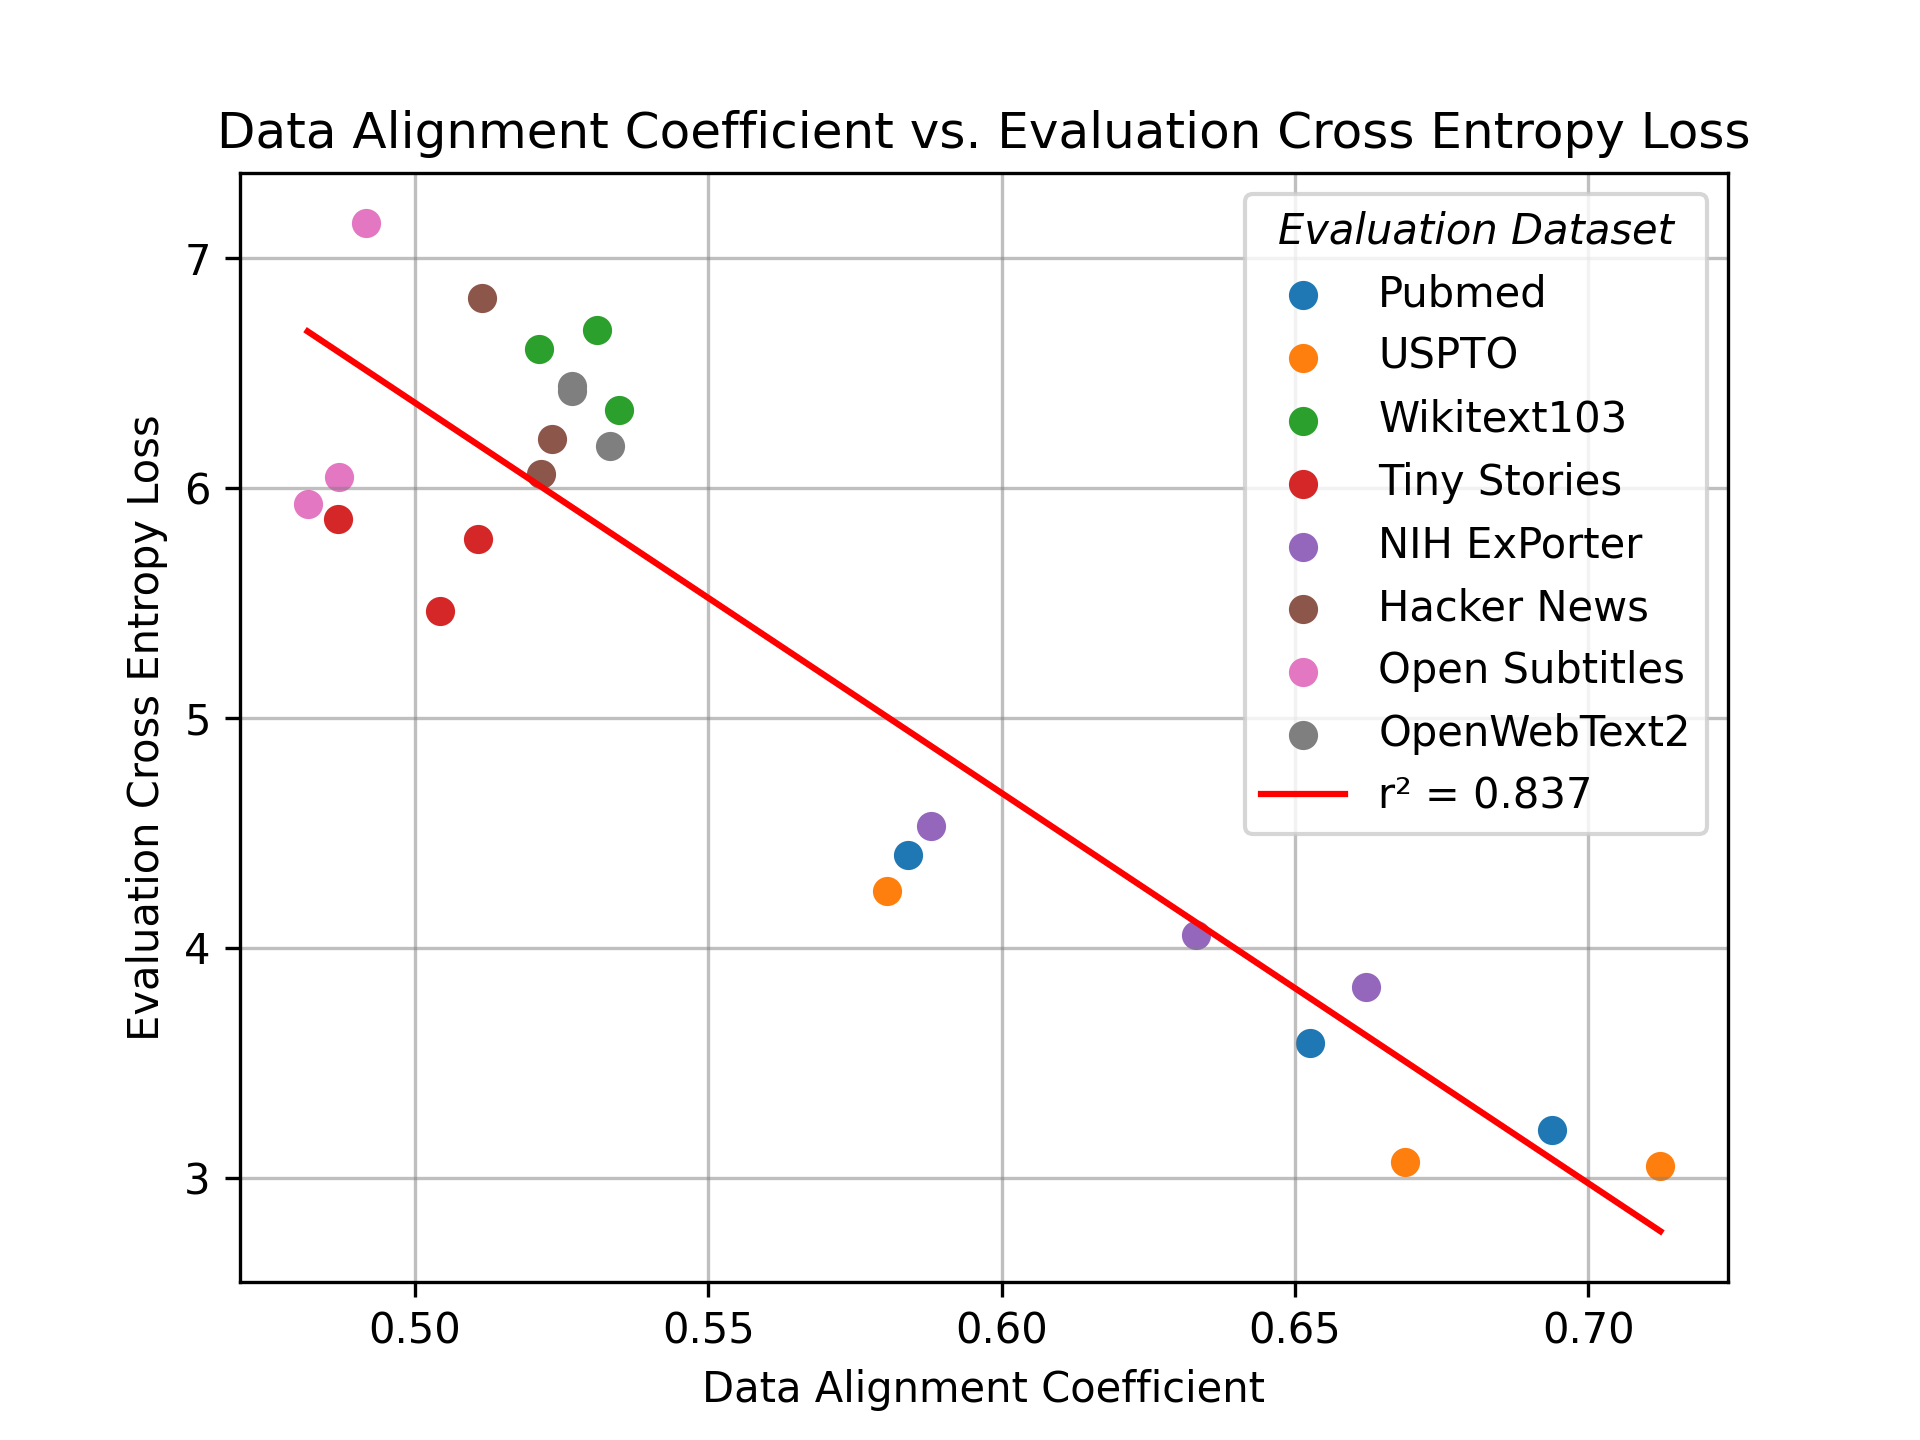
\includegraphics[scale=.85]{plots/align_loss_f.png}
%     \caption{ \textbf{The data alignment coefficient demonstrates a strong relationship with model performance (cross entropy loss) on various evaluation datasets ($r^2 = 0.837$)}. The data alignment coefficient is computed between a model's pre-training dataset (PubMed Abs., USPTO, or PubMed Abs. + USPTO) and a single evaluation dataset (represented by a unique color).
%     }
%     \label{fig:align_corr}
% \end{figure}

% OLD FIGURE. DELETED
% \begin{figure}
%     \centering
%     \includegraphics[scale=.85]{plots/align_loss_line.png}
%     \caption{\textbf{The data alignment coefficient demonstrates a solid relationship to model performance (cross entropy loss) on various evaluation datasets.}. Alignment coefficients below $\approx 0.55$ appear to be fairly noisy or even slightly positively correlated with performance (lower CE loss). But, with differences in alignment of $>0.1$ and, particularly, alignment coefficients $>0.575$, there appears a clear and strong positive relationship between the alignment coefficient and performance (lower CE loss).
%     The data alignment coefficient is computed between a model's pre-training dataset (PubMed Abs., USPTO, or PubMed Abs. + USPTO) and a single evaluation dataset (represented by a unique color).}
%     \label{fig:align_corr}
% \end{figure}
%%%%%%%%%%%%%%%%%%%%%%%%

%%%%%%%%%%%%%%%%%%%%%%%%
\begin{figure}
    \centering
    \title{Selected Experimental Model Completions}
    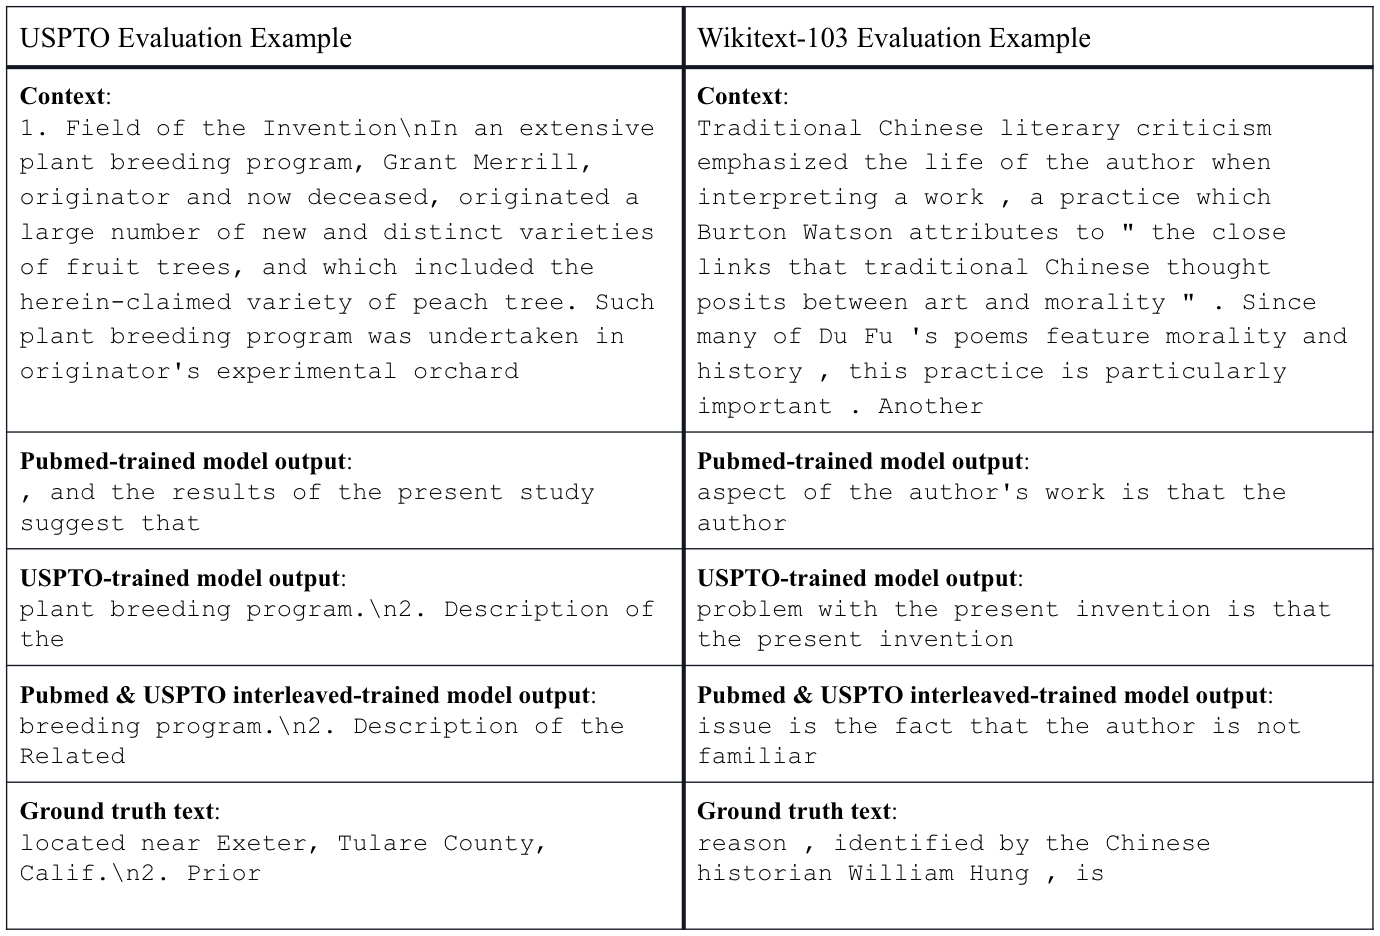
\includegraphics[scale=.28]{plots/model_outputs2.png}
    \caption{\textbf{Despite smaller scale (51M parameters) and relatively high loss/perplexity on certain evaluation datasets, the experimental models still grasp important aspects of sentence syntax and structure, even on evaluation data they otherwise struggle on (e.g. Wikitext-103, for which all models scored around 6.6 loss or more)}. In addition, when evaluated on similar, well aligned datasets (e.g. USPTO + PubMed Abs. (train) on USPTO (validation)), models are sometimes also able to match the form and semantic content of the example. Input examples were randomly picked from the given evaluation dataset.}
    \label{fig:outputs_are_good_despite_high_loss}
\end{figure}



%%%%%%%%%%%%%%%%%%%%%%%%

% \begin{table}
% \caption{\textbf{The data alignment coefficient appears to capture an intuitive notion of data similarity, since it finds training data that shares similar semantics and structure as the validation data as most aligned.} 
% In particular, PubMed Abs. (train) and NIH Exporter, which share the semantics of health-related research and the structure of being research writing, are found to be more aligned than USPTO (patent application backgrounds). 
% Similarly, USPTO + PubMed Abs. (train) is more aligned to USPTO (validation) than PubMed Abs. (train), but less aligned to USPTO (validation) than USPTO (train), as expected. Each cell indicates the alignment coefficient between the given pre-training dataset (row label) and evaluation dataset (column label).}
% \resizebox{\textwidth}{!}{%
% \centering
% \label{fig:align_table}
% \title{Data Alignment Coefficients between Training and Evaluation Data}
% \begin{tabular}{@{}lccccccccc@{}}
%         \toprule
%         Pre-training dataset & USPTO (validation) & PubMed Abs. (validation) & Openwebtext2 & NIH Exporter & Hacker News & Open Subtitles & Wikitext-103 & Tiny Stories \\
%         \midrule
%         USPTO & $0.7123 \pm 0.001717$ & $0.5840 \pm 0.001389$ & $0.5267 \pm 0.001377$ & $0.5879 \pm 0.001388$ & $0.5234 \pm 0.001275$ & $0.4917 \pm 0.001162$ & $0.5311 \pm 0.001303$ & $0.5107 \pm 0.001203$ \\
%         PubMed Abs. & $0.5805 \pm 0.001396$ & $0.6939 \pm 0.001697$ & $0.5268 \pm 0.001367$ & $0.6622 \pm 0.001569$ & $0.5114 \pm 0.001300$ & $0.4817 \pm 0.001145$ & $0.5212 \pm 0.001200$ & $0.4868 \pm 0.001167$ \\
%         USPTO + PubMed Abs. & $0.6687 \pm 0.001602$ & $0.6526 \pm 0.001513$ & $0.5332 \pm 0.001390$ & $0.6331 \pm 0.001452$ & $0.5215 \pm 0.001272$ & $0.4871 \pm 0.001123$ & $0.5347 \pm 0.001290$ & $0.5042 \pm 0.001169$ \\
%         \bottomrule
% \end{tabular}
% }
% \end{table}

\section{Using the Diversity Coefficient in Practice: Setting Batch Size and Network Parameters}
\label{body:div_parameters}
\textbf{Experiments:}
We test the sensitivity of the computed diversity coefficient value to changes in batch size and probe network parameters in order to gauge how these parameters should be set in practice for natural language datasets. 

We vary the batch size and observe the impact on the diversity coefficient. 
For the same number of batches (200) and probe network (pretrained, fine-tuned GPT-2), we computed the diversity coefficient of C4 for batch sizes of 128, 256, 512, and 1024, and plot the results in Figure \ref{fig:batchsize_network_experiments} (left).

We test the following probe network configurations to measure the diversity coefficient of C4 and of WikiText-103:
1. Pretrained GPT-2 with fine-tuning,
2. Pretrained GPT-2 without fine-tuning,
3. Randomly initialized GPT-2 with fine-tuning,
4. Randomly initialized GPT-2 without fine-tuning.
% % \begin{itemize}[topsep=-5pt, itemsep=-5pt, leftmargin=*] % use this if moved to main body
% \begin{itemize}
%     \item Pretrained GPT-2 with fine-tuning
%     \item Pretrained GPT-2 without fine-tuning
%     \item Randomly initialized GPT-2 with fine-tuning
%     \item Randomly initialized GPT-2 without fine-tuning
% \end{itemize}
Since using a random and/or non fine-tuned network is more resource efficient and easily accessible in practice, our motivation is to assess the necessity of using pre-trained and fine-tuned probe network, which is the original configuration used for Task2Vec in \cite{task2vec}. 
We aim to determine if a good approximation of diversity can be computed without fine-tuning. 
This setting is shown in Figure \ref{fig:batchsize_network_experiments} (right).

\begin{figure*}[h]
    \centering
    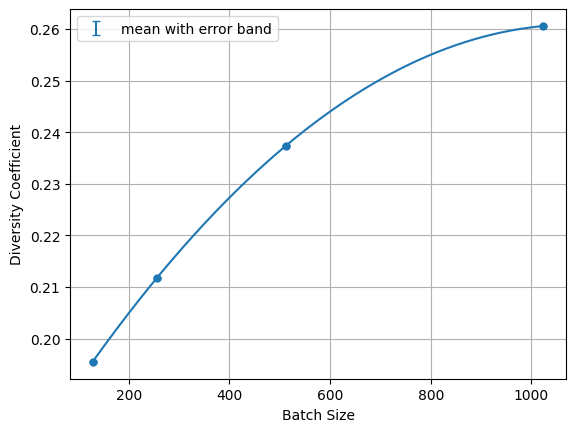
\includegraphics[width=0.49\linewidth]{plots/bs_curve.png}
    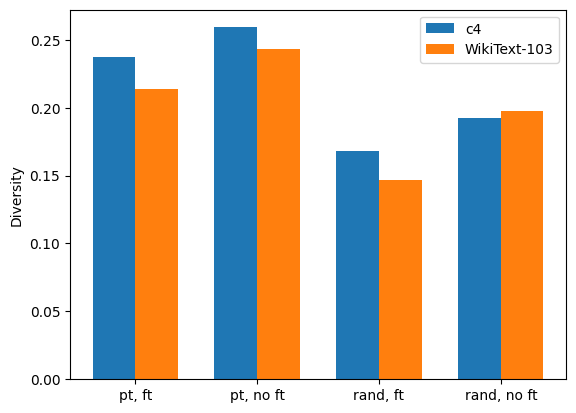
\includegraphics[width=0.49\linewidth]{plots/barplot_200tasks_bs512_diffmodel.png}
  \caption{\textbf{Diversity coefficients of C4 computed using different task batch sizes show positive and diminishing returns with increasing batch size (left). Diversity coefficients of C4 and WikiText-103 computed using different GPT-2 probe network configurations show that random networks' estimates likely diverge from those of pretrained networks (in particular, they appear to underestimate diversity), and non-finetuned networks overestimate diversity vs. finetuned networks (right).} 95\% confidence intervals for diversity coefficients are plotted, but are so small that they do not show. "pt" refers to pretrained network and "rand" refers to randomly initialized network. "ft" refers to a network that was finetuned per task and "no ft" refers to no finetuning performed.}
  \label{fig:batchsize_network_experiments}
\end{figure*}

\textbf{Results:} We observe that
\begin{itemize} %% use this if moved to main body
% \begin{itemize}
    \item \textbf{Diversity coefficient increases with task batch size, but with diminishing returns.} 
    Figure \ref{fig:batchsize_network_experiments} (left) shows positive correlation between the diversity coefficient and batch size. 
    This may be because larger batch sizes enable more unique tokens per batch.
    % , which may result in higher distances between batches. 
    % \item However, we observe diminishing returns to the increase in diversity coefficient with increasing batch size. 
    % We hypothesize that as the batch size continues to increase, there is greater coverage in data set properties like tokens, topics etc.
    % We hypothesize that as the batch size continues to increase, there is greater coverage in tokens, topics, document formats, etc. between batches, so the increase in the diversity coefficient saturates.
    \item \textbf{Coefficients from using random probe networks likely diverge from using pre-trained networks.} 
    Since the Task2Vec method \citep{task2vec} uses a pretrained fine-tuned network, we consider the diversity computed using this configuration as a source of truth. 
    Figure \ref{fig:batchsize_network_experiments} (left) shows that using a random probe network underestimates diversity compared to pretrained networks, which is in accordance with results from \cite{diversity} on vision datasets and indicative of random networks' estimates diverging from pre-trained networks'. 
    % We hypothesize that for random networks, the probe network parameters are not as calibrated to performing autoregressive language modeling, so batch representations from model parameters are similar, and the diversity is underestimated compared to pretrained networks.
    \item \textbf{Using a non-fine-tuned pre-trained network overestimates diversity.} 
    % Since the network is not fine-tuned, the activations may not represent a good learning of the batches.
    % This may introduce greater variability in the probe network activations between batches, so pairs of batches have higher Task2Vec (cosine) distance than batches embedded by fine-tuned networks. 
    % Lightly fine-tuning (the final layer \cite{task2vec}) of the probe network ensures the final Task2Vec embedding is more faithful to the dataset in question, as it adjusts the batch/task representation to a more similar distribution.
    % This is due to batches---while different content-wise---being conditioned on the same dataset.
    % On the other hand, a non-fine-tuned network may have more variable representations across batches, as it is not well-adapted to the dataset. 
    % This may explain the overestimation of the diversity coefficient that we observe.
    \item Trends in diversity coefficient overestimation vs. underestimation for different probe network configurations are consistent across C4 and WikiText-103.
\end{itemize}
Based on these findings, we recommend using a batch size of 512 sequences for faster computations and fewer out of memory issues and pre-trained fine-tuned network.
Since the other setting's diversity difference is large from the ground truth \cite{task2vec}, we can't recommend it. 
If the intuitive properties reproduce for the other two options, we'd recommend it, but this is left for future work.  
% Based on these findings, we recommend using a batch size of 512 sequences for faster computations and fewer out of memory issues. 
% We conjecture that our proposed diversity coefficient can be computed more efficiently using random and non fine-tuned networks, as eliminating pre-training and fine-tuning saves computational costs. 
% While the absolute diversity coefficient values differ compared to values computed using a pre-trained and fine-tuned network, this is not a serious issue as long as the same network configuration is used consistently  (see section \ref{appendix:discussion_cont}).
% Further validation is required to determine if indeed forgoing pre-trained and/or fine-tuned probe networks can produce as robust embeddings as the original Task2Vec method.

\section{Experimental Details}
\label{appendix:experiment_details}

\subsection{Dataset Preprocessing}
In accordance with \cite{task2vec}, we used the training split of datasets to finetune the probe network when computing Task2Vec embeddings per dataset. Sequences were tokenized using a pre-trained HuggingFace GPT-2 tokenizer based on byte-level Byte-Pair-Encoding, and padded or truncated to a max length of $128$. Because the WikiText-103 dataset contained empty text examples, we removed these examples before sampling batches to compute embeddings. 

\subsection{Model Architecture and Finetuning} 
We used a pre-trained GPT-2 model with a language modeling (LM) head on top. The pre-trained GPT-2 model itself has 12 layers, 12 heads, 768-d hidden size, and 117M total parameters. The LM head is a linear layer with weights corresponding to the input embedding layers. The model was pre-trained on the English language and the pre-trained GPT-2 tokenizer has a vocab size of $\approx$ 50k tokens. For all finetuning experiments, we fine-tuned only the LM head for 10 epochs. We used no learning rate scheduler and no gradient accumulation. We used the AdamW optimizer, since AdamW has been shown empirically to give better training loss and improved generalization.

We note that, in principle, the Task2vec diversity coefficient can be computed with any LLM. The metric itself is not specific to any particular LLM architecture or model version. We chose GPT-2 for our experiments due to computational efficiency and resource constraints. However, more powerful LLMs like LLaMA can also be used to compute the diversity coefficient. As long as the probe network used is consistent across experiments, the relative differences in the diversity coefficient value between datasets are directly comparable. The same goes for using pretrained vs. non-pretrained probe networks.

\subsection{Number of Batches and Batch Size Selection}
\label{appendix:parameter_selection}
Diversity coefficients in Table \ref{tab:div} were computed using randomly selected batches of size 512 sequences and a pre-trained, finetuned GPT-2 probe network. Diversity coefficients of C4, WikiText-103, The Pile, Pile-CC, HackerNews, NIH ExPorter, PubMed Abstracts, and USPTO were each computed using 200 sampled batches. Given resource constraints, we found 200 batches\footnote{This results in $(200^2-200)/2 = 19,900$ pairwise distances used to compute the diversity coefficient.} to be a sufficiently large number of batches to estimate the diversity coefficient with tight 95\% confidence intervals on the order of $1\text{e-}5$. We chose 512 as the batch size, since it is a relatively large and feasible batch size to fine-tune the probe network on 200 batches using Azure NV12s\_v3 instances equipped with Tesla M60 GPUs in a reasonable amount of time (30+ hours). 

\subsection{Diversity Coefficient Computation of Concatenated Datasets}
\label{appendix:concat_datasets}
The diversity coefficient of a concatenated dataset of C4 and WikiText-103 was measured over a combined set of batches.
Each batch consisted of sequences sampled from one of these datasets, e.g. a batch could have sequences randomly sampled from C4 \underline{or} WikiText-103 but not both.
The coefficient was computed over 400 batches of batch size 512 (200 batches from each dataset). 
Note that for the concatenated dataset, we utilized the same 200 batches per dataset that were used to compute the coefficients of C4 and of WikiText-103 individually.

The diversity coefficient of concatenated five sub-datasets of The Pile was computed over 1000 batches (200 batches from each dataset) of batch size 512. 
Similarly to the concatenated dataset of C4 and WikiText-103, we utilized the same 200 batches per dataset that were used to compute the coefficients of each individual sub-dataset.


\subsection{Diversity Coefficient of The Pile vs. Concatenation of Five Sub-Datasets}
We make a clarification on the approach taken to evaluate the diversity coefficient for The Pile vs. for concatenation of its five sub-datasets. 

The diversity coefficient of The Pile was computed over 200 batches sampled across all 22 sub-datasets of The Pile.
This means that any given batch could contain sequences across all 22 sub-datasets, i.e. a batch could have sequences from Pile-CC, HackerNews, and NIH ExPorter.

The diversity coefficient of the concatenated dataset was computed over 1000 batches comprised of 200 batches separately sampled from each of the five sub-datasets. 
Each batch contained sequences from only one sub-dataset, i.e. a batch could only have sequences from Pile-CC \underline{or} HackerNews \underline{or} NIH ExPorter.

We hypothesize this distinction in the diversity coefficient computation explains why the concatenated dataset has higher diversity, even though it consists of only five of the 22 sub-datasets of The Pile. 
For the diversity coefficient of The Pile, because batches were sampled such that any batch contains sequences from across the 22 sub-datasets, the batch representations learned by the probe network may have been more similar, resulting in lower diversity relative to the concatenated dataset.

\subsection{Details on Mixes used for Interleaved Datasets}
\label{appendix:mixdetails}

"C4 and WikiText-103 (Mix1)" denotes an interleaved dataset, i.e. a dataset where examples from each sub-dataset are randomly mixed together according to their proportion in the mix, so that if you iterate through each example in a 1:1 mix then you might see e.g. Dataset1 example, Dataset2 example, Dataset1 example, Dataset1 example, Dataset2 example. Mix1 indicates that this interleaved dataset is 75\% C4 examples and 25\% WikiText-103 examples.\\

"Combination of five datasets (Mix2)" also denotes an interleaved dataset. Mix2 indicates that each sub-dataset constitutes X\% of the interleaved dataset, where X\% is chosen to as closely match LLaMAv1's data training mix as possible. For example, if LLaMAv1 is composed of twice as much web crawl data as Wikipedia data, then our Mix2 will have 2 Pile-CC examples per 1 WikiText-103 example.\\

\section{Pairwise Distance Distributions of C4, WikiText-103, and The Pile}
\begin{figure}[h]
\centering
    \includegraphics[width=0.35\linewidth]{plots/histogram_div_C4.png}
    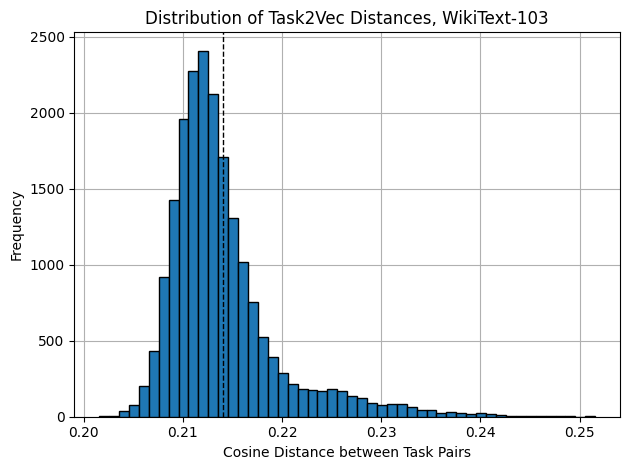
\includegraphics[width=0.35\linewidth]{plots/histogram_div_wikitext.png}
    \begin{center}
        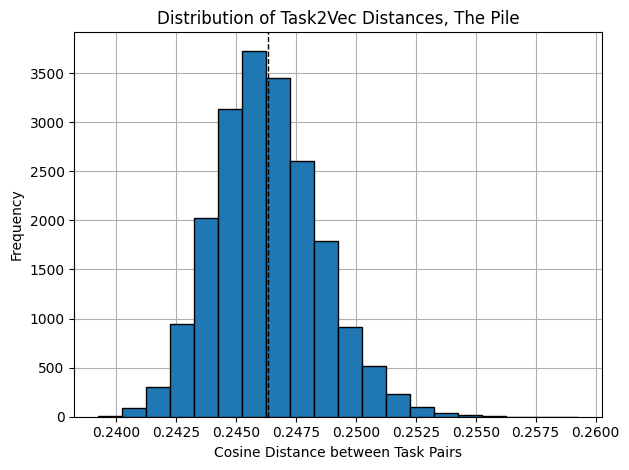
\includegraphics[width=0.35\linewidth]{plots/histogram_div_thepile.png}
    \end{center}
  \caption{\textbf{Distributions of pairwise batch distances from C4 (top left), WikiText-103 (top right), and The Pile (bottom) are approximately Gaussian, which justifies the use of a sample of batches to measure the diversity coefficient.} Dotted lines indicate the average distance, i.e. the diversity coefficient, for each dataset.}
  \label{fig:hist_indiv_data}
\end{figure}

\textbf{Experiments:}
To provide confidence in the magnitude of the coefficient values of C4, WikiText-103, and The Pile, we plot the distribution of distances per dataset in Figure \ref{fig:hist_indiv_data}. 
We aim to show that a subsample of batches can provide a good estimation of population statistics, such as the diversity coefficient, which measures the expected Task2Vec (cosine) distance between batches.

\textbf{Results:} 
% gitst: our plots are gaussian ==> we can make strong assumptions about the population ==> so we can use the mean + only 500 tasks which is less than C64_5 = 7624512 = infinity (say if there are 64 classes and 5-way) but see curse_dim for concreteness. 
For each dataset, the pairwise distances take on unimodal and approximately Gaussian distributions with few outliers. 
These results suggest the Task2Vec distances are approximately normally distributed.
This suggests we can make strong inferences about the population.
Specifically, we are able to compute a good estimate of the diversity coefficient using 200 batches using the mean.
This is in fact the same argument from \cite{curse_low_div}---but we verified it applied in our setting.
Figure \ref{fig:hist_indiv_data} also shows few outlier batches---the presence of which could influence the computed diversity coefficient.
This provides further confidence in the coefficient values computed and justifies our use of a sample of batches to estimate diversity.

% 4. the choice of using the expectation was empirically based on the bell shape of the histogram that shows the distribution of task distances (via Task2Vec) in figures \ref{hist_resnets_divs_cifarfs}, \ref{hist_resnets_divs_mi} \ref{hist_resnets_divs_gau}.
% They were Gaussian shaped, so the expectation of task distances was a sufficient statistic.
% 5. Although there are a large number of possible tasks based on combinatorial arguments (e.g. $C^{64}_{5} =7624512$), 500 samples are enough to make strong statistical inferences about the population. 
% If we assume the distribution of the data is Gaussian, then we expect to see a single mode with an approximate bell curve. 
% If we plot the histogram of task pair distances of the 500 tasks and see this, then we can infer our Gaussian assumption is approximately correct. 
% Given that the histograms in figure \ref{hist_resnets_divs_cifarfs}, \ref{hist_resnets_divs_mi} \ref{hist_resnets_divs_gau} appear Gaussian, we can infer our assumption is approximately correct. 
% This implies we can make strong statistical assumptions about the population – in particular, that we have a good estimate of the diversity coefficient using 500 samples.
% 6. The heat maps for MiniImagenet and Cifar-fs were homogeneous (uniform color) as shown in figures \ref{heat_map_resnets_divs_cifarfs},\ref{heat_map_resnets_divs_mi}, \ref{1d_gaussian_heatmaps}.
% % g. Finally, showing the histograms and heat maps of task distances shows the distribution of distances between tasks and it is impossible to summarize the distribution metric we used 


% You can have as much text here as you want. The main body must be at most $8$ pages long.
% For the final version, one more page can be added.
% If you want, you can use an appendix like this one, even using the one-column format.
%%%%%%%%%%%%%%%%%%%%%%%%%%%%%%%%%%%%%%%%%%%%%%%%%%%%%%%%%%%%%%%%%%%%%%%%%%%%%%%
%%%%%%%%%%%%%%%%%%%%%%%%%%%%%%%%%%%%%%%%%%%%%%%%%%%%%%%%%%%%%%%%%%%%%%%%%%%%%%%


% %%%%%%%%%%%%%%
% \begin{table}[t]
% % \caption{\textbf{Diversity coefficients of LLM pre-training datasets with 95\% confidence intervals are 3-5 times higher than the conceptual lower bound and more than half that of the upper bound.}}
% % \caption{\textbf{The data mixture affects the diversity of coefficients of LLM pre-training data sets, favoring the most intuitively diverse data set in the mix---common crawls like data.}
% % We discover that biasing the mixture towards wiki-text (more specialized topics) lowers the diversity compared to when the mixture is biased towards a more intuitively diverse data set, like common crawl type data sets (like C4).
% % This might explain why methods like DoReMi put the highest weight automatically on the most diverse data set (common crawl like data).
% % We report 95\% confidence intervals.}
% \caption{\textbf{The data mixture affects the diversity of coefficients of LLM pre-training data sets, where combining data sets increases the diversity.}
% We discover common crawl type data sets (like C4) tend to have a high diversity on their own but their diversity can be increased by combining it with other type of data.
% This might explain why methods like DoReMi put the highest weight automatically on the most diverse data set (common crawl like data).
% We report 95\% confidence intervals.}
% \vskip 0.15in
% \begin{center}
% \begin{small}
% \begin{sc}
% \begin{tabular}{lcccr}
% \toprule
% Dataset & Diversity Coeff. \\
% \midrule
% Lower Bound (LB) & $\textbf{0.0525}\pm 3.41\textrm{e-}4$ \\

% WikiText-103 & $0.202 \pm 1.03\textrm{e-}3$ \\ % https://wandb.ai/brando/beyond-scale/runs/c88ozru5/overview?workspace=user-brando
% C4 & $0.228 \pm 1.02\textrm{e-}3$ \\ % https://wandb.ai/brando/beyond-scale/runs/6mrvh267/overview?workspace=user-brando

% % WikiText-103 & $0.2140 \pm 7.93\textrm{e-}5$ \\
% % C4 & $0.2374 \pm 2.785\textrm{e-}5$ \\

% C4 and WikiText-103 (Mixture Uniform [0.5, 0.5]) & $ 0.236 \pm 1.07\textrm{e-}3 $\\ % https://wandb.ai/brando/beyond-scale/runs/z7yg6lz1/logs?workspace=user-brando
% C4 and WikiText-103 (Mixture DoReMi [0.89, 0.11]) & $0.229 \pm 1.02$\textrm{e-}3 \\ % https://wandb.ai/brando/beyond-scale/runs/muidji30/overview?workspace=user-brando
% C4 and WikiText-103 (Mixture LLaMA v1 [0.77, 0.23]) & $0.227 \pm 1.04\textrm{e-}3$\\ % https://wandb.ai/brando/beyond-scale/runs/e9ic8ov1/overview?workspace=user-brando

% C4 and WikiText-103 (Mixture 1:2 [0.25, 0.75]) & $ \textbf{0.244} \pm 1.010\textrm{e-}3 $\\ % https://wandb.ai/brando/beyond-scale/runs/g6heox73/overview?workspace=
% C4 and WikiText-103 (Mixture 2:1 [0.75, 0.25]) & $0.235 \pm  1.04$\textrm{e-}3\\ % https://wandb.ai/brando/beyond-scale/runs/i29297m2/overview?workspace=user-brando

% Upper Bound (UB) & $\textbf{0.4037} \pm 1.932\textrm{e-}5$ \\
% \bottomrule
% \end{tabular}
% \label{table:div}
% \end{sc}
% \end{small}
% \end{center}
% \vskip -0.1in
% \end{table}
% %%%%%%%%%%%%%%


\textbf{OpenWebtext: } 
Data from Reddit post URLs was extracted, deduplicated, and filtered for English content using FastText. Web pages were pulled using the newspaper python package, and near-duplicates were identified and removed using local-sensitivity hashing (LSH). Only documents with a unique content similarity of less than 0.5 and more than 128 tokens were retained. The finalized dataset comprises 38GB from 8,013,769 documents. Annotations: None present in the dataset.
Used to train GPT2.

%%%

\section{Generative IN-Context Learning (GINC) Dataset}
\label{appendix:ginc}
\subsection{Background}
The GINC dataset is generated using the latent concept framework proposed in \cite{ginc}, where language models condition on a prompt to infer latent document concepts learned during pre-training. The pretraining distribution is defined using a uniform mixture of Hidden Markov Models (HMMs) parameterized over a family $\Theta$ of latent concepts.

\subsection{Definitions of GINC Dataset Parameters}
\textbf{Number of latent concepts:} A latent concept $\theta$ parameterizes the transitions of a HMM in the mixture. A latent concept (e.g. a wiki bio) contains document statistics, such as semantics, syntax, and the formatting of and distribution of tokens.

\textbf{Vocabulary size:} Each HMM in a given mixture outputs a fixed number of tokens, defined as the vocabulary size. The vocabulary is generated by enumerating combinations of letters from a to z, aa to az, etc. The delimiter token is designated by a backslash. Sequences are tokenized by whitespace.

%In experiments, all other GINC parameters are kept the same (e.g. experiments conducted comparing diversity coefficient vs. number of latent concepts only vary the number of latent concepts in each generated GINC dataset).

\subsection{Supplemental Figures for Diversity Coefficient vs. GINC Parameters}
\begin{figure*}[h]
\centering
    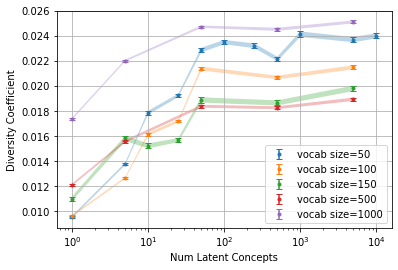
\includegraphics[width=0.45\linewidth]{plots/div_nlatents.png}
    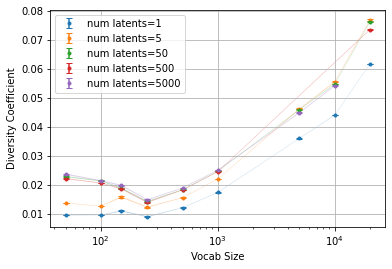
\includegraphics[width=0.45\linewidth]{plots/div_vocab.png}
  \caption{\textbf{Trends noted in Section \ref{body:ginc} are consistent for diversity coefficient vs. number of latent concepts (left) and coefficient vs. vocab size (right) when the other parameter changes.} The diversity coefficient with 95\% confidence intervals saturates with increasing number of latent concepts (left) even as vocab size is varied between 50-1000. Larger vocab sizes generally produce higher diversity coefficients (right) even as the number of latent concepts is varied between 1-5000.}
  \label{fig:div_vs_nlatents_vocab}
\end{figure*}

Figure \ref{fig:div_vs_nlatents_vocab} confirms that the trends between the diversity coefficient and number of latent concepts (left) hold even as vocab size is varied.
Similarly, trends between the diversity coefficient and the vocabulary size (right) hold as the number of latent concepts is varied. 
These trends were noted in Section \ref{body:ginc}.

\section{Discussion (cont.)}
\label{appendix:discussion_cont}
% - However, it is worth noting that our metric relies on tunable parameters, including the number of batches, batch size, and probe network depth. 
% 	- These parameters affect the absolute value of the diversity coefficient, necessitating recalibration of the conceptual lower and upper bounds accordingly (see sections \ref{appendix:parameter_selection} and \ref{appendix:div_parameters}).
% 		- However, this can be resolved by using a consistent choice of hyper parameters. 
% 		- In addition, while we employ a pre-trained and fine-tuned network as a probe, we are actively exploring alternative approaches, such as using random and/or non-fine-tuned networks (see section \ref{appendix:div_parameters}).
% - how does diversity relate to quality/performance?
% 	- diversity might not help models e.g. just uniform noise has the most diversity (NFT)
% 	- however, since diversity tries to capture spread, a higher diversity (with a sufficiently large model) likely leads to better performance and therefore your data is of higher quality. 
% - diversity hides truly causual stuff, but this was by design to make it more practical usable
% 	- but you can do abalation experiments like we did
% 	- but it's more widely useful/applicable
% 	- no silver bullet
% - However, the bounds we propose only apply to sequence data with a symbolic vocabulary.
% 	- However, using a multimodal embedding method that is used to embed diversity coefficients and the lower/upper bounds across tasks would aid in usage of these bounds across modalities.
% 		- but we hypothesize that CLIP/aligned embeddings are enough. Coming up with a L/U bound for vision can be useful to further validate/test/examine our currently proposed methods
% - To really clarify why FIM is better than activations we provide this intuitive explanation. FIM gives a weight/feature of which parameter of the generative distribution matters (e.g. the first coordinate of Task2Vec corresponds to how artsy the text sequence is,). This is a feature of a task or dataset itself. Therefore, FIM exactly approximate the (task) data generative distribution we are trying to embed. Therefore, it results in superior representations for datasets compared to activations since it directly approximates the data (or task) generative distribution. 

Our paper introduces a metric that leverages tunable parameters, such as the number of batches, batch size, probe network configuration (pre-trained vs. random, fine-tuned vs. not) and depth. 
While these elements influence the diversity coefficient's absolute value and necessitate the recalibration of lower and upper bounds (see Appendices \ref{appendix:parameter_selection} and \ref{body:div_parameters}), a consistent choice of hyperparameters can mitigate these effects. 

Intriguingly, our proposed diversity may not always correlate with model performance, as high diversity could simply be due to uniform noise. 
Nevertheless, we contend that a higher diversity, in the context of a sufficiently large model, likely indicates superior performance and data quality. 
Furthermore, our diversity metric is intentionally designed to be widely applicable, albeit concealing causal factors, rendering it an effective tool for ablation studies.
% Investigating the relation between diversity and performance, it is worth noting that the highest diversity may not always correspond to the highest performance. However, in an adequately large model, increased diversity may signify improved performance and data quality. 

Despite our diversity metric's broader applicability, it may obscure certain causal factors. 
This limitation is intentional to enhance its practical usage---since causality is often difficult to infer and is out of scope.
This can be overcome with data property ablation studies, as we showed in our GINC dataset experiments. 

Currently, our proposed bounds are specific to sequence data with a symbolic vocabulary, limiting their applicability across different modalities. 
To overcome this limitation, we suggest using a multimodal embedding method for embedding diversity coefficients and lower/upper bounds across tasks.

% The superiority of FIM over activations can be explained by its ability to provide a weight for each parameter of the generative distribution, resulting in more effective dataset representations.
To really clarify why FIM is better than activations, we provide this intuitive explanation. FIM gives a weight/feature of which parameter of the generative distribution matters, 
e.g. the first coordinate of Task2Vec corresponds to how artsy the text sequence is. 
This is a feature of a task or dataset itself. Therefore, FIM exactly approximates the (task) data generative distribution we are trying to embed. 
Therefore, we conjecture it results in superior representations for datasets compared to activations since it directly approximates the data (or task) generative distribution.
Our study, and references, provide positive evidence in favor of this argument.

The strength of embeddings is their ability to approximate \textbf{semantics} in a way that symbols may struggle with, such as distinguishing the equivalence of two sentences with different symbols but identical meanings. 
In NLP there is no easy way to determine this equivalence. In formal mathematics, symbolic semantics and thus equivalence can sometimes be done exactly. 
Though it does not come without its costs, e.g. requires expert knowledge, computationally demanding or (approximately) exhaustive representations like e-graphs. 
Therefore, embedding methods for data diversity, quality, etc. have the unique advantage of being more generally applicable. 

Our diversity calculations predominantly utilize a small model (GPT-2). 
Despite the ongoing discussion concerning the emergence of large language models (LLMs), our conjecture extends the results to models of all sizes. 
We base this inference on the fact that the manifestation of emergence is intimately tied to the specific metric employed, and the sudden unpredictable jumps disappear when smooth metrics are applied \cite{schaeffer2023emergent}.
The cosine distance is smooth and does not have this issue. 

% \textbf{Why and when does diversity matter?}
% We conjecture two main reasons why diversity matters and explain our rationale:
% \begin{enumerate}
%     \item \textbf{Conjecture 1: Diversity matters because it enables learning-to-learn (proxy for General Intelligence).}
%     This is the main conjecture we provide evidence in this paper. 
%     The main argument is that if there is high diversity, it means there are many tasks in the dataset.
%     Therefore, for the model to do well, it has to do well on all tasks.
%     One way to do it is by learning-to-learn and therefore transfer when challenged with solving a new task. 
%     An alternative would be memorizing all the tasks. 
%     \item \textbf{Conjecture 2: Diversity matters because it increases changes that training set covers test set.}
%     Diversity is a formalization of coverage---it aims to be the effective (average) number of tasks in a dataset.
%     Therefore, the higher the diversity, the more tasks a dataset has.
%     This (might) increase the probability that the training set covers the test set and improves performance.
%     This exploration of this conjecture is left for future work. 
% \end{enumerate}
\textbf{Why and when does diversity matter?}
We propose two central conjectures for the importance of diversity and provide the underlying rationale:
\begin{enumerate}
    \item \textbf{Conjecture 1: Diversity is essential because it promotes learning-to-learn (a surrogate for General Intelligence).} 
    The main argument is that a significant level of diversity corresponds to a multitude of tasks in the dataset.
    Therefore, to achieve high (test) performance, the model must perform well on all tasks.
    One potential strategy is by learning-to-learn, thereby allowing transferability when tasked with a new problem. 
    Another alternative could be to memorize all tasks. 
    \item \textbf{Conjecture 2: Diversity is crucial because it enhances the probability that the pre-training set covers the test set.}
    Diversity is a formal score of coverage---it aims to reflect the effective number of tasks in a dataset.
    Thus, increased diversity equates to more tasks in a dataset.
    This (could) boosts the chance of the training set covering the test set, hence improving performance, given a sufficiently large model like an LLM.
    The direct exploration of this conjecture is slated for future investigation, but we provide a suggestive (correlative) analysis of one reason why LLMs might perform so well. 
\end{enumerate}

Another benefit is that our method does not rely on activations from an arbitrarily selected layer in a network.
Lastly, note that activations may be unreliable for embedding dataset/tasks because large distances between datasets/tasks may be due to well-separated decision boundaries instead of intrinsic semantic properties of the dataset/task.
In contrast, the diversity coefficient is well-justified, extensively tested in our work and previous work, e.g. the diversity coefficient correlates with ground truth diversities, cluster according to semantics, taxonomy etc. (see section \ref{appendix:ground_truth_div} and \cite{task2vec, curse_low_div}). 
In short, FIM-based representations are motivated by information theory (e.g. FIMs are metrics in distributions) and have been extensively tested by independent sources \citep{curse_low_div, task2vec, nlp_task2vec}.

Data has taken a central role in the success of modern machine learning methods, like GPT4 \cite{gpt4}, CLIP \cite{clip}, and PaLM 2 \cite{google2023palm2}, with special relevance for architectures with few inductive biases, like the popular Transformer \citep{vaswani2017attention}.
Therefore, it is paramount to understand the pretraining data we use, beyond scale alone.
We conclude the diversity coefficient is a trustworthy metric, and conjecture the diversity coefficient can be used to build quality, diverse datasets for LLMs.
We hope our contributions inspire more effective data collection and curation in machine learning that goes beyond scale alone to improve performance. 


% % let's address reviewers suggestions:
% % While the authors acknowledge that the metric may
% % obscure certain causal factors, they do not provide a thorough analysis of the potential limitations of the metric.
% % Additionally, the authors do not provide a detailed discussion of the potential implications of their findings for future
% % research in the

% \subsubsection{Limitations}
% % hides causual factors
% % perhaps expensive due to task2vec, fim, but not worse than vendi
% % Unclear if expectation is best aggregation metric, perhaps we do want the size to be a part of the metric?
% \textbf{}

% \subsubsection{Implication}
% % quantatitive ways to access data quality and data coverage
% % the more diverse the data set the higher the chance the test set is covered, so better data sets can be use
% % automatic ways to calculate diversity
\textbf{Limitations:}
\begin{itemize}
    \item The diversity coefficient presents an aggregate measure that masks the underlying causal factors. 
    Despite this, we illustrate how it might be employed to uncover these factors.
    We show this through the use of vocabulary size and latent space, acknowledging that these experiments could be resource-intensive.
    Causality is a challenging topic, and we do not claim to solve it through our experiments. 
    Our experiments in this regime are mostly to show that the diversity coefficient (might) correlates/captures different sources of diversity beyond number of concepts or tasks.
    \item The computation of Task2Vec embeddings requires more resources than computing simply the activations. 
    However, given the proven correlation with ground truth task generative parameters from previous studies, we posit that it supersedes activations. 
    Furthermore, we hypothesize that using activations could result in high distances due to optimization for decision boundaries, making it less reliable for measuring distances 
    i.e., high distances in activation space might be artificially high.
    We observed this but plan to give more detailed study in the future. 
    \item The choice of an expectation as the aggregation function could be seen as arbitrary. 
    Alternatives such as the Vendi score are promising, but still under-explored and computationally demanding compared to expectations/sums. 
    Future work could focus on the comparative analysis of the total distance sum and the Vendi score. 
    We hypothesize, in line with the Central Limit Theorem (CLT), that the results might not differ significantly e.g., CLT still converges to (unit) Normal given the proper normalization procedure. 
    \item We reject the notion that the use of models is a limitation. 
    As discussed earlier, models can provide superior data embeddings, and all forms of data representations are always required.
    For example, the identity function or symbols are data representations.
\end{itemize}

\textbf{Implications:}
\begin{itemize}
    \item Given the impressive performance of LLMs, our study suggests a correlation with our diversity measure, potentially providing an explanation for this high level of performance.
    \item High diversity implies a larger task coverage. 
    Therefore, we conjecture that a highly diverse pre-training set could increase the probability of including relevant pre-training data for the target task/testing.
    This suggests that collecting more diverse data could be a method to enhance performance.
    If the model is sufficiently large, we conjecture this method always (stochastically) monotonically increases the performance (as implied by \citep{zhang2021understanding}).
    \item The transition from a qualitative to a quantitative measure of diversity can be seen as a significant advancement in the field because of conceptual transitions about how we think and talk about data quality/diversity.
    \item The use of Task2Vec to embed data implies a method applicable to any modality, potentially benefiting all areas of machine learning research.
\end{itemize}

Importantly, the relationship between pre-training dataset diversity and test performance remains a key question.
% We observe a negative correlation between diversity and perplexity, i.e., an increase in diversity correlates with a decrease in perplexity---indicating a positive relationship between diversity and model performance (although the perplexity values are large). Therefore, we conjecture diversity improves test performance on general tasks.
To investigate, we conduct preliminary experiments, pre-training three GPT-2 models on datasets of varying diversities, then evaluate their performance on diverse validation datasets.
% We observe in table \ref{tab:div_vs_ppl} a negative correlation between diversity and perplexity, i.e., an increase in diversity correlates with a decrease in perplexity---indicating a positive relationship between diversity and model performance (although the perplexity values are large). 
We observe in Table \ref{tab:div_vs_ppl} that increased diversity leads to decreased cross-entropy loss, indicating a positive relationship between diversity and model performance on diverse tasks. Although the cross-entropy values are arguably large, Figure \ref{fig:outputs_are_good_despite_high_loss} shows that even the smallest 51M parameter models were still pre-trained enough to grasp important aspects of sentence syntax and structure of their respective dataset, indicating model performance on evaluation represents meaningful improvements in ability. 
Hence, we conjecture pre-training on higher diversity data improves test performance on diverse tasks, though more extensive experiments are needed to know so conclusively.
% However, this type of experiment is challenging because pre-training an LLM at scale is expensive---more than 10M dollars \cite{ruiz2023train}.

\subsection{Future Work}
Our future research will explore the potential of the Task2Vec distance function for pre-training dataset curation. 
Given that the objective of pre-training is to maximize downstream task performance, we define high-quality training data as data that facilitates the best achievable performance on such tasks.
We anticipate that higher diversity in the dataset will increase the likelihood of achieving this objective.  
The rationale is that a higher data diversity implies a broader coverage of tasks or batches, thereby increasing the probability of training the model on tasks or data representations that are relevant to evaluation tasks.
Our focus will be to leverage Task2Vec to assess the similarity between individual data points, batches, or datasets to a target task. 
This assessment will enable us to curate the training data by selectively removing tasks that resemble random, noisy, or irrelevant sequences, which may adversely affect downstream performance.




% \section{Impact Statement}
% % DEFAULT: This paper presents work whose goal is to advance the field of Machine Learning. There are many potential societal consequences of our work, none which we feel must be specifically highlighted here.
% This paper presents work whose goal is to advance the field of machine learning, and, in particular, presents tools for better understanding and training large language models (LLMs) via a rigorous approach to data quality. One important societal consequence of this is the fact that a better understanding of data quality would allow researchers and practitioners to make more informed decisions on dataset selection and more efficiently train LLMs. Thus, by reducing the need for the scaling of data quantity, this would likely lead to lower model development and inference costs, thereby making the development and use of LLMs more affordable and widely accessible to researchers and practitioners. Furthermore, more efficient training would lead to lower energy expenditure during model development, partially ameliorating any environmental degradation resulting from energy production and use. Finally, a rigorous understanding of data quality yields greater transparency about the value of data corpora, thereby allowing for fairer and better-grounded trade and arbitration with regard to the buying and selling of corpora. Aside from these factors, there are surely many other potential societal and ethical consequences of our work, but there are no others which we feel must be specifically highlighted here.











